% ============================================================================
% An Adaptive LLM-Assisted Knowledge-Based System for Payroll Tax Calculation Under Retroactive Changes in
% Government Regulations and Company Policies
%
% IEEE Access manuscript. Build in v2/paper/:
%   pdflatex main && bibtex main && pdflatex main && pdflatex main
% Data figures: env\Scripts\python v2\paper\make_figures.py (reads the analysis files under v2/work).
% ============================================================================
% ieeeaccess.cls redefines the TeX primitive \year, which pgf reads while loading; the primitive is restored
% while TikZ loads.
\let\primitiveyear\year
\documentclass{ieeeaccess}
\let\accessyear\year
\let\year\primitiveyear
\usepackage{tikz}
\let\year\accessyear
% pgf overwrites \pdfpageresources; the template's spot color space (used by the blue figure and table labels)
% is registered again through pgf's own resource list.
\makeatletter
\expandafter\pgfutil@addpdfresource@colorspaces\expandafter{\the\PANTONE}
\makeatother
\usetikzlibrary{arrows.meta,positioning,fit,calc,shapes.geometric}
\usepackage{cite}
\usepackage{amsmath,amssymb,amsfonts}
\usepackage{algorithm}
\usepackage{algorithmic}
\usepackage{graphicx}
\usepackage{textcomp}
\usepackage{xcolor}
\usepackage{booktabs}
\usepackage{array}
\usepackage{tabularx}
\usepackage{multirow}
\usepackage{url}
\providecommand{\nolinkurl}[1]{\url{#1}}

\newcolumntype{L}{>{\raggedright\arraybackslash}X}
\newcolumntype{C}{>{\centering\arraybackslash}X}
\newcolumntype{P}[1]{>{\raggedright\arraybackslash}p{#1}}
\newcolumntype{R}[1]{>{\raggedleft\arraybackslash}p{#1}}

\newcommand{\K}{\mathcal{K}}
\newcommand{\SG}{S^{G}}

\definecolor{cai}{RGB}{226,135,30}
\definecolor{cdet}{RGB}{40,100,170}
\definecolor{chum}{RGB}{40,140,80}
\definecolor{cgr}{RGB}{140,140,140}
\definecolor{cred}{RGB}{200,50,50}
\definecolor{cpur}{RGB}{130,60,160}
\tikzset{
  b/.style={draw, rounded corners=2pt, align=center, font=\scriptsize, minimum height=0.8cm, inner sep=2pt},
  bai/.style={b, fill=cai!18, draw=cai},
  bdet/.style={b, fill=cdet!12, draw=cdet},
  bhum/.style={b, fill=chum!15, draw=chum},
  bsrc/.style={b, fill=white, draw=cgr},
  ar/.style={-{Stealth[length=1.6mm]}, semithick}
}
% TikZ diagrams of the manuscript. The values of the bitemporal example are engine output on the reference KB.

% ------------------------------------------------------------------------------------------- replay protocol
\newcommand{\figReplayProtocol}{%
\resizebox{0.97\textwidth}{!}{%
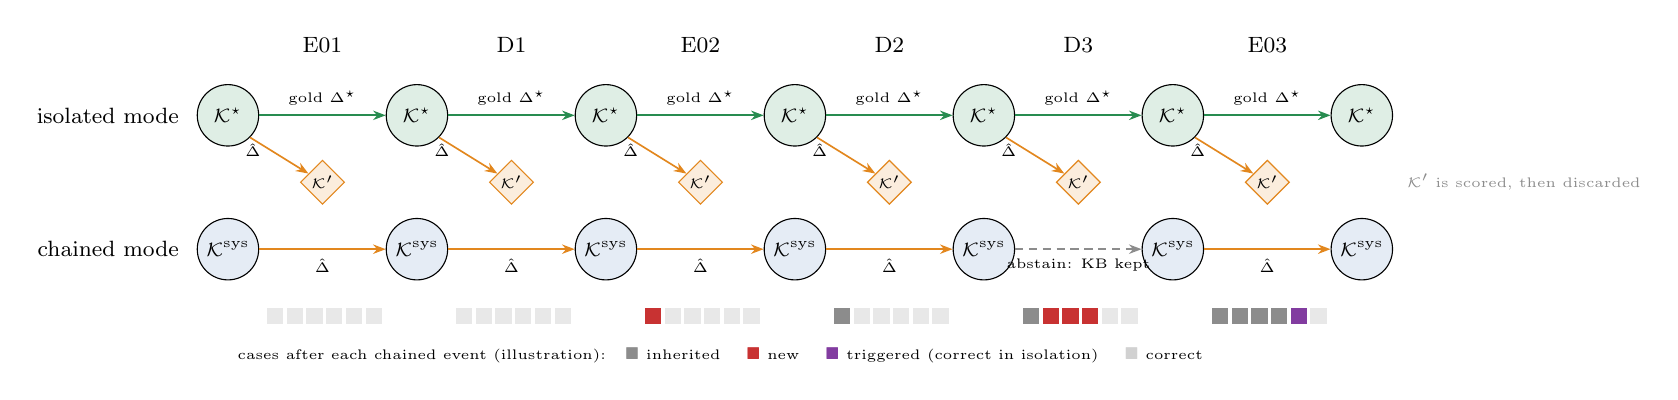
\begin{tikzpicture}[kb/.style={draw, circle, minimum size=0.78cm, font=\scriptsize, inner sep=0pt},
  sq/.style={minimum size=0.22cm, draw=white, line width=0.4pt, inner sep=0pt}]
\node[font=\footnotesize, anchor=east] at (-0.5,1.7) {isolated mode};
\node[font=\footnotesize, anchor=east] at (-0.5,0) {chained mode};
\foreach \lab [count=\i from 0] in {E01,D1,E02,D2,D3,E03}{
  \node[font=\footnotesize] at (\i*2.4+1.2,2.6) {\lab};
  \node[kb, fill=chum!15] (g\i) at (\i*2.4,1.7) {$\mathcal{K}^\star$};
  \node[kb, fill=cdet!12] (c\i) at (\i*2.4,0) {$\mathcal{K}^{\mathrm{sys}}$};}
\node[kb, fill=chum!15] (g6) at (14.4,1.7) {$\mathcal{K}^\star$};
\node[kb, fill=cdet!12] (c6) at (14.4,0) {$\mathcal{K}^{\mathrm{sys}}$};
\foreach \i [evaluate=\i as \j using int(\i+1)] in {0,...,5}{
  \draw[ar, chum] (g\i) -- node[above, font=\tiny, text=black]{gold $\Delta^\star$} (g\j);
  \node[draw=cai, fill=cai!15, diamond, inner sep=0.8pt, font=\tiny] (k\i) at (\i*2.4+1.2,0.85) {$\mathcal{K}'$};
  \draw[ar, cai] (g\i.south east) -- node[left, font=\tiny, text=black, pos=0.35]{$\hat\Delta$} (k\i);}
\foreach \i [evaluate=\i as \j using int(\i+1)] in {0,1,2,3,5}{
  \draw[ar, cai] (c\i) -- node[below, font=\tiny, text=black]{$\hat\Delta$} (c\j);}
\draw[ar, cgr, densely dashed] (c4) -- node[below, font=\tiny, text=black]{abstain: KB kept} (c5);
\node[font=\tiny, text=cgr, anchor=west] at (14.85,0.85) {$\mathcal{K}'$ is scored, then discarded};
\foreach \i/\cols in {0/{cgr!20,cgr!20,cgr!20,cgr!20,cgr!20,cgr!20}, 1/{cgr!20,cgr!20,cgr!20,cgr!20,cgr!20,cgr!20},
  2/{cred,cgr!20,cgr!20,cgr!20,cgr!20,cgr!20}, 3/{cgr,cgr!20,cgr!20,cgr!20,cgr!20,cgr!20},
  4/{cgr,cred,cred,cred,cgr!20,cgr!20}, 5/{cgr,cgr,cgr,cgr,cpur,cgr!20}}{
  \foreach \c [count=\k from 0] in \cols {\node[sq, fill=\c] at (\i*2.4+0.6+\k*0.25,-0.85) {};}}
\node[font=\tiny, anchor=west] at (0,-1.35) {cases after each chained event (illustration):\quad
  \textcolor{cgr}{$\blacksquare$} inherited \quad \textcolor{cred}{$\blacksquare$} new \quad
  \textcolor{cpur}{$\blacksquare$} triggered (correct in isolation) \quad \textcolor{cgr!40}{$\blacksquare$} correct};
\end{tikzpicture}}}

% ------------------------------------------------------------------------------------------- architecture
\newcommand{\figArchitecture}{%
\resizebox{0.95\textwidth}{!}{%
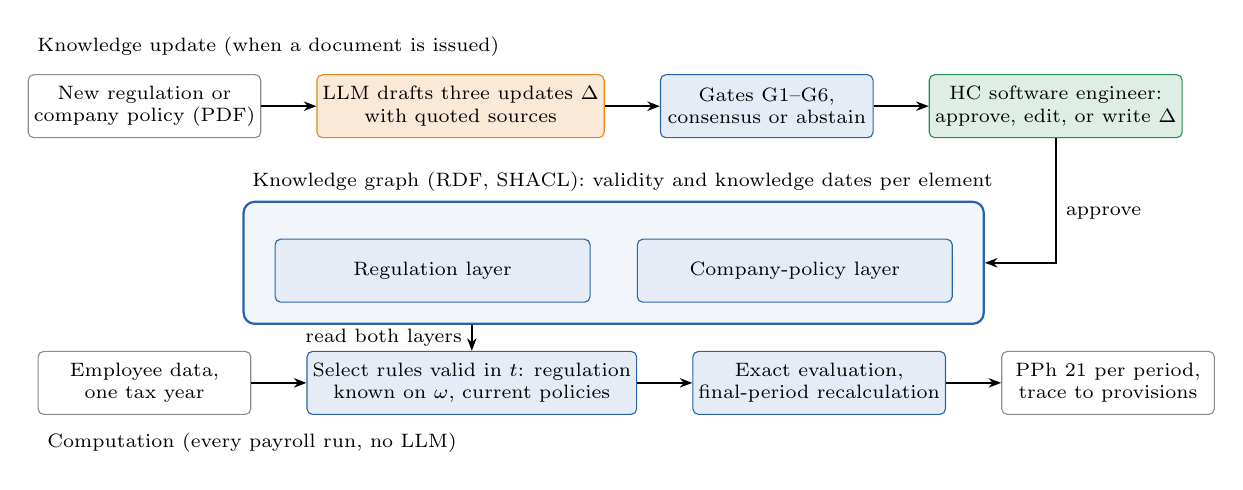
\begin{tikzpicture}[node distance=5mm and 7mm]
\node[bsrc, minimum width=2.7cm] (doc) {New regulation or\\company policy (PDF)};
\node[bai, right=of doc, minimum width=2.7cm] (llm) {LLM drafts three updates $\Delta$\\with quoted sources};
\node[bdet, right=of llm, minimum width=2.7cm] (gate) {Gates G1--G6,\\consensus or abstain};
\node[bhum, right=of gate, minimum width=2.7cm] (rev) {HC software engineer:\\approve, edit, or write $\Delta$};
\draw[ar] (doc)--(llm); \draw[ar] (llm)--(gate); \draw[ar] (gate)--(rev);
\node[draw=cdet, fill=cdet!6, thick, rounded corners, minimum width=9.4cm, minimum height=1.55cm,
  below=12mm of $(llm)!0.5!(gate)$] (kb) {};
\node[bdet, minimum width=4cm] at ($(kb.center)+(-2.3,-0.1)$) {Regulation layer};
\node[bdet, minimum width=4cm] at ($(kb.center)+(2.3,-0.1)$) {Company-policy layer};
\node[font=\scriptsize, anchor=south west] at (kb.north west) {Knowledge graph (RDF, SHACL): validity and
  knowledge dates per element};
\draw[ar] (rev.south) |- node[pos=0.3, right, font=\scriptsize]{approve} (kb.east);
\node[bsrc, below=27mm of doc, minimum width=2.7cm] (emp) {Employee data,\\one tax year};
\node[bdet, right=of emp, minimum width=2.7cm] (sel) {Select rules valid in $t$: regulation\\known on $\omega$, current policies};
\node[bdet, right=of sel, minimum width=2.7cm] (calc) {Exact evaluation,\\final-period recalculation};
\node[bsrc, right=of calc, minimum width=2.7cm] (out) {PPh 21 per period,\\trace to provisions};
\draw[ar] (emp)--(sel); \draw[ar] (sel)--(calc); \draw[ar] (calc)--(out);
\draw[ar] (kb.south -| sel.north) -- node[left, font=\scriptsize]{read both layers} (sel.north);
\node[font=\scriptsize, anchor=west] at ($(doc.north west)+(0,0.35)$) {Knowledge update (when a document is issued)};
\node[font=\scriptsize, anchor=west] at ($(emp.south west)+(0,-0.35)$) {Computation (every payroll run, no LLM)};
\end{tikzpicture}}}

% ------------------------------------------------------------------------------------------- bitemporal
\newcommand{\figBitemporal}{%
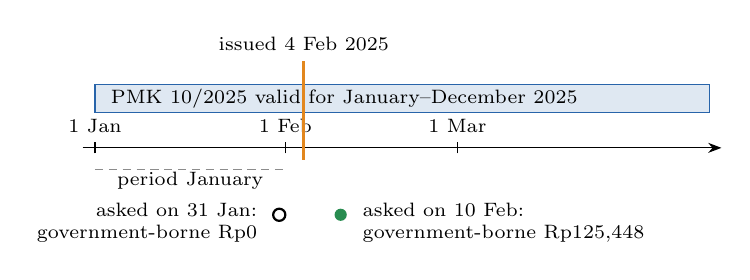
\begin{tikzpicture}[x=0.078cm]
\fill[cdet!15, draw=cdet] (0,1.05) rectangle (100,1.4);
\node[font=\scriptsize, anchor=west] at (1,1.225) {PMK 10/2025 valid for January--December 2025};
\draw[-{Stealth}] (-2,0.6) -- (102,0.6);
\foreach \x/\l in {0/1 Jan, 31/1 Feb, 59/1 Mar}{\draw (\x,0.53)--(\x,0.67) node[above, font=\scriptsize]{\l};}
\draw[cai, very thick] (34,0.45) -- (34,1.7) node[above, font=\scriptsize, text=black]{issued 4 Feb 2025};
\draw[densely dashed, cgr] (0,0.32) -- (31,0.32); \node[font=\scriptsize] at (15.5,0.18) {period January};
\fill[white, draw=black, thick] (30,-0.25) circle (2.2pt);
\node[font=\scriptsize, anchor=east, align=right] at (28,-0.35) {asked on 31 Jan:\\government-borne Rp0};
\fill[chum] (40,-0.25) circle (2.2pt);
\node[font=\scriptsize, anchor=west, align=left] at (42,-0.35) {asked on 10 Feb:\\government-borne Rp125,448};
\end{tikzpicture}}

% ------------------------------------------------------------------------------------------- acquisition flow
\newcommand{\figAcquisitionFlow}{%
\resizebox{0.95\textwidth}{!}{%
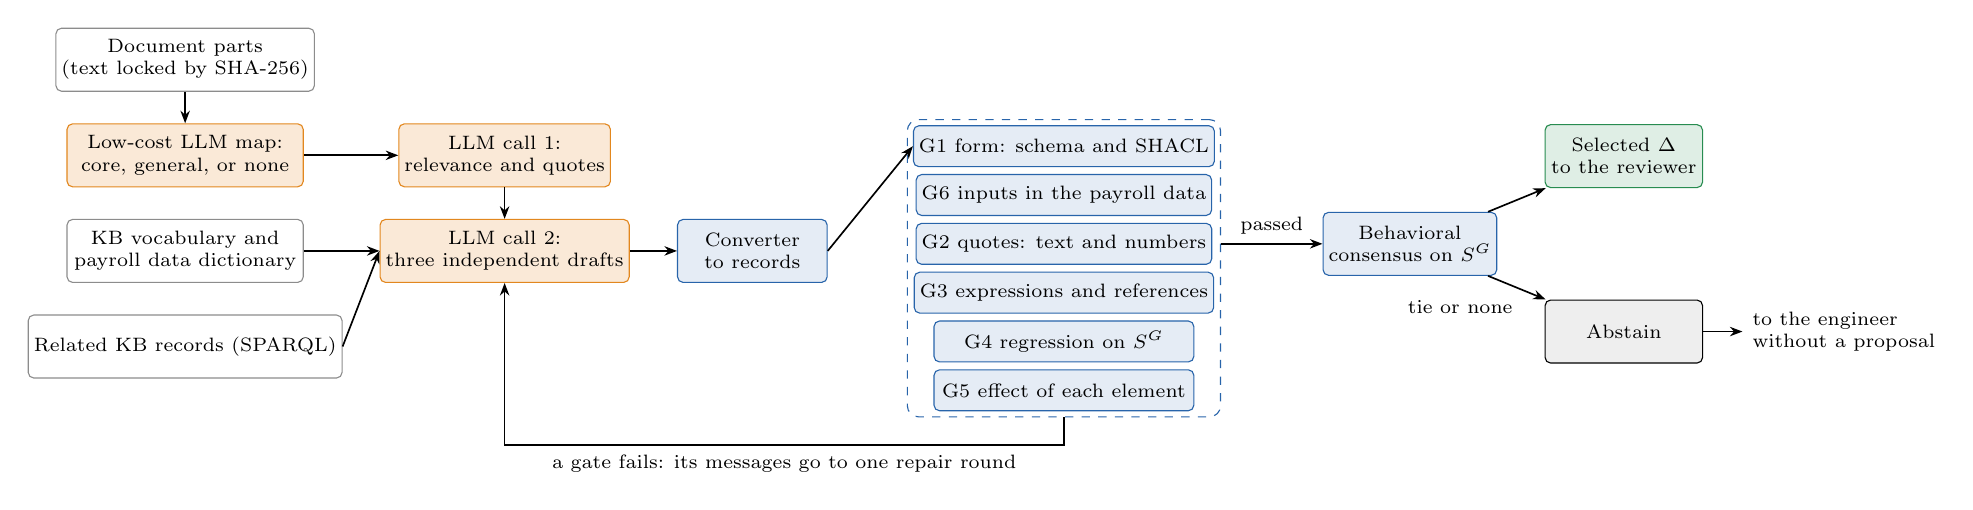
\begin{tikzpicture}[node distance=4mm and 6mm]
\node[bsrc, minimum width=3cm] (seg) {Document parts\\(text locked by SHA-256)};
\node[bai, below=of seg, minimum width=3cm] (tab) {Low-cost LLM map:\\core, general, or none};
\node[bsrc, below=of tab, minimum width=3cm] (voc) {KB vocabulary and\\payroll data dictionary};
\node[bsrc, below=of voc, minimum width=3cm] (rec) {Related KB records (SPARQL)};
\node[bai, right=12mm of tab, minimum width=2.5cm] (rel) {LLM call 1:\\relevance and quotes};
\node[bai, below=of rel, minimum width=2.5cm] (dr) {LLM call 2:\\three independent drafts};
\node[bdet, right=of dr, minimum width=1.9cm] (conv) {Converter\\to records};
\foreach \g/\n [count=\i] in {G1/form: schema and SHACL,G6/inputs in the payroll data,G2/quotes: text and numbers,
  G3/expressions and references,G4/regression on $S^G$,G5/effect of each element}{
  \node[bdet, minimum width=3.3cm, minimum height=0.52cm] (g\i) at ($(conv.east)+(3.0,1.95-\i*0.62)$) {\g\ \n};}
\node[draw=cdet, dashed, rounded corners, inner sep=2pt, fit=(g1)(g6)] (gates) {};
\node[bdet, right=14mm of g3, minimum width=2.2cm] (cons) {Behavioral\\consensus on $S^G$};
\node[bhum, above right=3mm and 6mm of cons, minimum width=2cm] (sel) {Selected $\Delta$\\to the reviewer};
\node[b, below right=3mm and 6mm of cons, minimum width=2cm, fill=cgr!15] (abs) {Abstain};
\draw[ar] (seg)--(tab); \draw[ar] (tab.east)--(rel.west); \draw[ar] (voc.east)--(dr.west);
\draw[ar] (rec.east)--(dr.west);
\draw[ar] (rel)--(dr); \draw[ar] (dr)--(conv); \draw[ar] (conv.east)--(g1.west);
\draw[ar] (gates.south) -- ++(0,-0.35) -| node[pos=0.25, below, font=\scriptsize]{a gate fails: its messages go to one repair round} (dr.south);
\draw[ar] (gates.east |- cons.west) -- node[above, font=\scriptsize]{passed} (cons.west); \draw[ar] (cons)--(sel); \draw[ar] (cons)--node[below left, pos=0.6, font=\scriptsize]{tie or none} (abs);
\draw[ar] (abs.east) -- ++(0.5,0) node[right, font=\scriptsize, align=left]{to the engineer\\without a proposal};
\end{tikzpicture}}}



\begin{document}
\bstctlcite{IEEEexample:BSTcontrol}
\history{Date of publication xxxx 00, 0000, date of current version xxxx 00, 0000.}
\doi{10.1109/ACCESS.2026.DOI}

\title{An Adaptive LLM-Assisted Knowledge-Based System for Payroll Tax Calculation Under Retroactive Changes in Government Regulations and Company Policies}

\author{\uppercase{Obi Kastanya}\authorrefmark{1},
\uppercase{Mahathir Muhammad}\authorrefmark{1},
AND \uppercase{Ratih Nur Esti Anggraini}\authorrefmark{1}}

\address[1]{Department of Informatics, Institut Teknologi Sepuluh Nopember, Surabaya 60111, Indonesia
(e-mail: 6025252015@student.its.ac.id; 6025252008@student.its.ac.id; ratih\_nea@if.its.ac.id)}
\tfootnote{This work received no external funding.}

\markboth
{Kastanya \headeretal: Adaptive LLM-Assisted Knowledge-Based System for Payroll Tax Calculation}
{Kastanya \headeretal: Adaptive LLM-Assisted Knowledge-Based System for Payroll Tax Calculation}

\corresp{Corresponding author: Ratih Nur Esti Anggraini (e-mail: ratih\_nea@if.its.ac.id).}

\begin{abstract}
Indonesian employers withhold employee income tax (PPh 21) monthly under rules that changed 13 times in 2023--2026, five of them retroactively. Calculators that hard-code these rules need new code for each change and cannot reproduce earlier results after a retroactive rule appears. This study presents an adaptive knowledge-based system that keeps these rules current with a large language model (LLM). Government regulations and each company's pay policies form two layers of one knowledge graph in which every rule records when it is valid and when it became known. A deterministic engine computes the tax from these records and recalculates paid months when a retroactive rule arrives. The LLM only drafts updates, each of which must quote its source and pass deterministic gates. The system abstains when the drafts disagree. The evaluation replayed the documents of five real companies with 13 regulations, 6 labor agreements, and 20 distractors and scored 26,328 payslips against a reference checked by a tax practitioner. With a human-capital software engineer approving the proposals, payslip accuracy on the payroll date was 0.945 to 1.000 in four companies and exceeded that of a code-based update made 26 days after each issue. An incomplete labor-agreement installation lowered the fifth company to 0.239, so the pre-specified pooled hypothesis failed. A completeness gate added after the evaluation removed this failure in a replay of the recorded drafts. The engineer wrote updates by hand for 11 of 138 documents. Every late upload of a retroactive rule left the earlier payroll reproducible.
\end{abstract}

\begin{keywords}
Bitemporal knowledge graph, knowledge acquisition, knowledge-based systems, large language models, payroll tax, retroactive regulation.
\end{keywords}


\titlepgskip=-21pt

\maketitle

% ============================================================================
\section{Introduction}
\label{sec:intro}
% ============================================================================
\PARstart{I}{ndonesian} employers compute and withhold Income Tax Article 21 (PPh 21) from the pay of each employee every month, so an error in the tax rules reaches every payslip of the company. These rules change often: 13 regulatory events changed the PPh 21 computation for permanent employees between 2023 and 2026, and seven of them were issued in 2025 (Fig.~\ref{fig:timeline}). Government Regulation (PP) 58/2023 and Minister of Finance Regulation (PMK) 168/2023 replaced the annualized monthly method with average effective rates (TER) from January 2024. Both were issued in the last week of December 2023~\cite{pp58_2023,pmk168_2023}. Five of the 13 events took effect retroactively. One of them is PMK 10/2025, which introduced government-borne tax (DTP) for employees in labor-intensive sectors. Because PMK 10/2025 was issued on 4 February 2025 but covers January 2025, a January payroll that was correct when it ran owed a correction a month later~\cite{pmk10_2025}.

\begin{figure*}[!t]
\centering
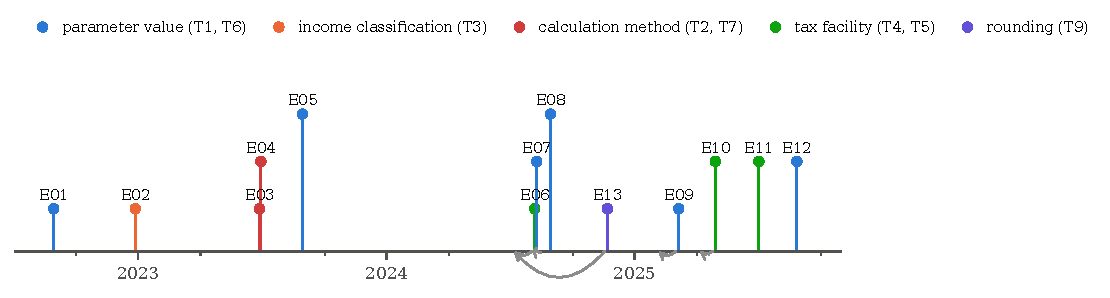
\includegraphics[width=\textwidth]{figs/fig_timeline.pdf}
\caption{Regulatory events that changed PPh 21 for permanent employees in 2023--2026, placed at their issue dates.}
\label{fig:timeline}
\end{figure*}

The government regulation is only one layer of the rules that a payslip follows. Each company adds its own pay policies on allowances, overtime, the religious holiday allowance (THR), and employer-borne tax through a collective labor agreement or company regulation. The same regulation therefore changes the payslips of two companies differently. A regulatory change can also silently alter the effect of a company clause.

Because payroll software usually encodes both layers in program code or spreadsheets~\cite{ramadhani2021grossup,kusuma2026pph21}, every change needs new code. The commit histories of two open-source PPh 21 calculators show that TER was added 26 and 915 days after PP 58/2023 was issued. A knowledge-based system (KBS) separates the rules from the code that executes them~\cite{merigoux2021catala}, but the work moves to keeping the knowledge base (KB) current. Large language models (LLMs) can turn legal text into structured rules~\cite{janatian2023texttostructure} although they are unreliable when asked to compute tax directly~\cite{nay2024taxattorneys,dahl2024legalfictions}.

Prior work leaves three gaps for a payroll system that must follow such a stream of changes.
\begin{enumerate}
  \item \emph{No LLM-assisted tax KB is maintained through a sequence of real changes.} Work that combines LLMs with tax rules formalizes the law at one point in time~\cite{veeramani2026neurosymbolic,lorenzo2025translating,jurayj2026tax}. The closest work updates a tax program by one legal year with LLM-written candidates and a majority vote~\cite{goganikhiabani2025maintaining}, without a chain of updates and without testing earlier periods.
  \item \emph{No executable tax KB handles retroactive rules together with company policies.} Versioned legal knowledge graphs record how the text of a norm evolves~\cite{demartim2025satgraph}, but their rules are not executed. Payroll and tax systems do not separate company policies from the regulation they build on~\cite{dumancic2021payroll,alhawari2026payroll}.
  \item \emph{No evaluation measures the payslips that result from LLM-drafted updates.} Existing studies score each drafted rule or answer on its own~\cite{goganikhiabani2025maintaining,jurayj2026tax}, not the payslips of a company that receives the updates one after another.
\end{enumerate}

This study addresses the three gaps with an adaptive KBS for PPh 21 (Fig.~\ref{fig:architecture}). The novelty of the system is an executable two-layer knowledge graph that LLM-drafted updates keep current and that records the legal validity of every rule and the date on which the rule became known. Deterministic gates check each drafted update before a behavioral consensus proposes it or abstains. A company therefore receives retroactive government regulations and changes of its own policies without any change of program code. A deterministic engine computes the tax. A software engineer who maintains the company's human capital (HC) systems such as payroll approves each proposal. The contributions of this study are as follows:
\begin{itemize}
  \item \emph{A two-layer bitemporal knowledge base with LLM-assisted updates.} Government regulations and company policies are separate layers of one RDF knowledge graph with executable rules. Their bitemporal records let the engine recalculate months already paid when a retroactive rule arrives while the earlier results stay reproducible. An update pipeline drafts each change three times from the document, checks every draft with six deterministic gates, and proposes an update only when the drafts agree.
  \item \emph{A chained, payslip-level evaluation on real document streams.} Five real companies with one installation each received the regulations of 2023--2026, their labor agreements, and distractor documents in the order of issue. Every payslip was scored against a reference knowledge base checked by a tax practitioner and compared with a code-based update made 26 days after each issue.
  \item \emph{Evidence on payslip accuracy and manual work.} Payslip accuracy on the payroll date exceeded that of the code-based update in four of the five companies when an HC software engineer approved the proposals. A completeness gate added after the evaluation brought the fifth company to the level of the code-based update in a replay of the recorded drafts. The engineer wrote updates by hand for 11 of the 138 documents.
\end{itemize}

Section~\ref{sec:background} summarizes PPh 21 and its changes, and Section~\ref{sec:related} reviews related work. Section~\ref{sec:system} describes the system and Section~\ref{sec:design} the evaluation, whose results are presented in Section~\ref{sec:results} and discussed in Section~\ref{sec:discussion} before Section~\ref{sec:conclusion} concludes the paper.

% ============================================================================
\section{Background: Payroll Income Tax in Indonesia}
\label{sec:background}
% ============================================================================
\subsection{Computing PPh 21 for a Permanent Employee}
\label{sec:pph21}
The monthly gross income of a permanent employee includes the salary, fixed allowances, irregular payments such as THR and bonuses, and benefits in kind, which have been taxable since July 2023. It also includes the premiums that the employer pays for work accidents, death, and health. Until 2023 the employer annualized each month's regular income and deducted the occupational expense, the employee's pension contributions, and the nontaxable amount (PTKP) of the employee's family status. The employer then taxed the result at the five progressive rates of 5\% to 35\% under Article 17~\cite{uu7_2021,pmk101_2016,per16_2016}. Since January 2024 the employer applies a monthly average effective rate (TER) to the gross income of January to November. The rate depends on the gross amount and on a category (A, B, or C) that follows from the PTKP status. In the final period the employer recomputes the tax of the whole year under Article 17 and withholds the difference from the amount already withheld~\cite{pp58_2023,pmk168_2023}. An employee with status K/1 and a monthly salary of Rp15,000,000 pays Rp933,660 in January 2024 at a TER of 6\% and Rp3,667,320 in March, when the THR doubles the gross income. The annual recomputation in December credits the earlier months and leaves Rp186,480 to withhold.

\subsection{Types and Dates of Rule Changes}
\label{sec:changes}
The corpus and the results are organized by the ten types of change of Table~\ref{tab:types}. Parameter changes (T1) are the most frequent among the real events, while company policies (T10) form the largest group of prospective units. Fig.~\ref{fig:timeline} places the 13 real regulations on a time axis with one color for each group of these types.

Two dates matter for every change. The issue date is the day on which the rule becomes known, whereas the start of validity is the day from which it binds. The start of validity of a tax facility such as DTP is the first tax period that it covers and can precede the date on which the regulation itself takes effect. The two dates coincide for most parameter changes. A retroactive rule separates them so that the correct withholding of a past month depends on the date on which the question is asked. The gray arrows of Fig.~\ref{fig:timeline} run from the issue date of each retroactive rule back to the start of its validity. The rounding rule of Director General Regulation PER-11/PJ/2025 is an example: it was issued in May 2025 for periods from January 2025. A KB that records only validity cannot reproduce what an employer should have withheld with the knowledge available at the time. A KB that records only the latest knowledge cannot report the correction owed for the months already paid.

\begin{table}[!t]
\caption{Types of change with their real events and prospective test units.}
\label{tab:types}
\centering\footnotesize
\setlength{\tabcolsep}{3pt}
\begin{tabularx}{\columnwidth}{@{}lLlr@{}}
\toprule
Code & Type of change & Real events & Units \\
\midrule
T1 & a single parameter value (wage cap, rate, ceiling) & E01, E05, E07, E08, E12 & 10 \\
T2 & a rate table is created or changed & E03 & 6 \\
T3 & income classification & E02, E04 & 6 \\
T4 & a new facility with eligibility criteria & E06, E11 & 7 \\
T5 & the scope of a facility & E10 & 6 \\
T6 & the validity period of a rule & E09 & 4 \\
T7 & a change of calculation method & E03, E04 & 3 \\
T8 & repeal without replacement & none & 3 \\
T9 & a calculation procedure such as rounding & E13 & 5 \\
T10 & a company policy & labor agreements & 30 \\
\bottomrule
\end{tabularx}
\end{table}

\subsection{Company Policies on Top of the Regulation}
\label{sec:policies}
Employers decide parts of the payroll themselves through company regulations or collective labor agreements. These parts include proration for partial months, the THR formula, overtime, allowances, and whether the employer bears the tax through a tax allowance (gross-up) or pays it directly. These policies form a second layer of rules that reads the values of the first and may not override mandatory provisions. A regulation can also apply differently across companies. PMK 10/2025 grants DTP only to employers whose business classification code is on its list. PP 7/2025 reduces the work-accident premium only for labor-intensive employers with at least 50 workers. The correctness of a payslip is therefore a property of each company because it depends on the regulation, the profile of the company, and the company's own policies taken together.

\subsection{Scope}
The study covers permanent employees of private and state-owned employers and tax years 2023--2026, with regulatory history from 2012 used for development. It excludes non-permanent workers, severance and other income taxed at final rates, and the filing of withholding slips.

% ============================================================================
\section{Related Work}
\label{sec:related}
% ============================================================================
Five lines of work meet in this study: rules-as-code systems, incremental knowledge acquisition, LLM-based formalization of law, the evaluation of repeated LLM updates, and temporal legal knowledge graphs.

\subsection{Rules as Code and Payroll Tax Systems}
Rules-as-code and payroll tax systems hold knowledge written by people. Catala translates statutes into a programming language with general cases and exceptions based on default logic and found bugs in an official implementation during its evaluation~\cite{merigoux2021catala,huttner2022catala}. DataLex~\cite{mowbray2023scaling,mowbray2023xai} and Logical English~\cite{kowalski2022logicalenglish} follow the same principle with rule languages close to legal text. OpenFisca indexes its tax parameters by the date from which they apply~\cite{openfisca}. For payroll, Dumancic et al.\ state payroll tax and social-security legislation declaratively for policy optimization~\cite{dumancic2021payroll}. Al-Hawari et al.\ build a rule-based payroll system~\cite{alhawari2026payroll}. Studies of PPh 21 describe mostly procedural systems~\cite{ramadhani2021grossup,yulistyawati2022payroll,kusuma2026pph21} and the overwithholding that TER produces on irregular income~\cite{sherra2025ter}. None of these systems evaluates updates written by a machine.

\subsection{Incremental Knowledge Acquisition}
Ripple-Down Rules add a rule whenever an expert finds a wrong case and use cornerstone cases to keep the new rule from breaking cases that were already right~\cite{compton2021rdr}. The regression gate G4 of this study plays the role of the cornerstone cases. Work on legal logic formalizes changes of law and theory revision with temporalized revision operators~\cite{moguillansky2024temporalised}. An expert still writes every change in this line of work.

\subsection{LLMs for Legal and Tax Formalization}
LLM-based formalization of legal and tax text targets the law as it stands at one time. LLMs have turned legal text into structures for legal expert systems~\cite{janatian2023texttostructure}. Veeramani et al.\ let an LLM extract the Indian Income Tax Act into a knowledge graph for a symbolic rule engine and report 80\% accuracy of the combined system on 20 scenarios~\cite{veeramani2026neurosymbolic}. Yadamsuren et al.\ formalize one section of the United States Internal Revenue Code in Prolog to detect a known inconsistency~\cite{yadamsuren2026formalization}. Lorenzo et al.\ benchmark the translation of French tax provisions into Catala by code similarity and syntactic validity without executing the output~\cite{lorenzo2025translating}. Jurayj et al.\ combine an LLM with a Prolog solver on 100 tax cases, where o3 gives 75 correct answers, 15 wrong answers, and 10 abstentions without gold statutes~\cite{jurayj2026tax}. LLM performance on tax law improves across model generations without reaching expert level~\cite{blairstanek2023gpt3,nay2024taxattorneys}. Commercial legal research tools also still hallucinate~\cite{magesh2025hallucination}.

The nearest exception is the work of Gogani-Khiabani et al., who ask an LLM to update United States tax code from 2020 to 2021 and select candidates by behavioral majority vote~\cite{goganikhiabani2025maintaining}. Their accuracy with the previous year's code as context ranges from 21\% to 100\% for GPT-3.5 and from 48\% to 100\% for GPT-4.0. Their study covers one step, does not test earlier periods, and does not measure error propagation. The consensus of this system uses the same selection idea and adds verification gates and abstention.

\subsection{Repeated LLM Updates and Their Evaluation}
Sequential knowledge editing degrades a language model after many edits~\cite{gupta2024editing}. KoLEG keeps performance above 95\% after four cumulative edits from Korean legal amendments~\cite{seo2025koleg}, but it edits the model and not a rule base. Prior et al.\ consolidate four German statutes with an LLM and report that exact match falls from 50.3\% for a single amendment to 20.51\% for amendment chains~\cite{prior2025risks}. Their object is XML text rather than executed rules, and only the final version of each chain is compared.

Self-consistency~\cite{wang2023selfconsistency} and CodeT~\cite{chen2023codet} choose among sampled outputs by their agreement or by generated tests. Selective prediction evaluates a model that may abstain by its risk and coverage~\cite{geifman2017selective,xin2021abstention}. The consensus and the abstention of this study follow these two ideas, which have not been applied to an executable, time-versioned legal rule base.

\subsection{Temporal Legal Knowledge Representation}
Work on temporal legal knowledge representation versions data or norms but does not evaluate machine-written updates of executed rules. Bitemporal databases separate the time in which a fact is valid from the time at which it was recorded~\cite{snodgrass1999developing}. SQL:2011 standardizes both time axes~\cite{kulkarni2012temporal}. De Martim models norms as works with versioned expressions so that answers are not anachronistic~\cite{demartim2025satgraph}. Kharraz et al.\ define conflicts in a temporal normative logic~\cite{kharraz2024conflicts}, and Governatori and Rotolo model the abrogation and annulment of norms in defeasible logic~\cite{governatori2010changing}.

The European Legislation Identifier (ELI)~\cite{publicationsoffice2026elien}, OWL-Time~\cite{cox2017owltime}, PROV-O~\cite{lebo2013provo}, and LegalRuleML~\cite{palmirani2021legalruleml} provide vocabularies for documents, time, provenance, and norms. This study reuses all of these vocabularies except LegalRuleML, together with the Shapes Constraint Language (SHACL) for validation~\cite{knublauch2017shacl}. Metamorphic testing of tax software~\cite{tizpaz2023metamorphic} informs the test design of Section~\ref{sec:design}.

\subsection{Positioning}
The closest work differs from this study in the properties that Table~\ref{tab:position} compares. Rules-as-code systems execute the law but are written and maintained by people. LLM-based formalization drafts rules but at one point in time and without a company layer. Versioned legal graphs follow the law through time but do not execute it. No work in the table keeps an executable rule base current through a sequence of machine-drafted updates that includes retroactive rules and company policies, and none scores the outputs that a company receives after each update. A dash in the table marks a property that is absent or not reported as a focus of the cited publication.

\begin{table*}[!t]
\caption{Position of this study relative to the closest work.}
\label{tab:position}
\centering\footnotesize
\setlength{\tabcolsep}{3pt}
\begin{tabularx}{\textwidth}{@{}P{3.1cm} P{1.8cm} L P{1.5cm} P{1.6cm} P{1.5cm} P{1.3cm} P{1.2cm} P{2.0cm}@{}}
\toprule
Work & Domain & Representation & Knowledge author & Sequence of updates & Retroactive rules (knowledge date) & Company layer & Abstains & Evaluation \\
\midrule
Catala~\cite{merigoux2021catala,huttner2022catala} & tax and benefits & domain-specific language & people & -- & -- & -- & -- & bugs in an official implementation \\
DataLex~\cite{mowbray2023scaling,mowbray2023xai} & legislation & rule language and inference engine & people & -- & -- & -- & -- & -- \\
Dumancic et al.~\cite{dumancic2021payroll} & payroll & formal model compiled to constraints & people & -- & -- & -- & -- & use at an agency \\
Ripple-Down Rules~\cite{compton2021rdr} & general & rules with exceptions & expert & yes & -- & -- & -- & cornerstone cases \\
Veeramani et al.~\cite{veeramani2026neurosymbolic} & Indian income tax & knowledge graph and symbolic rules & LLM and expert & proposed & -- & -- & -- & 20 scenarios \\
Lorenzo et al.~\cite{lorenzo2025translating} & French tax & Catala & LLM & -- & -- & -- & -- & code similarity \\
Jurayj et al.~\cite{jurayj2026tax} & US tax & Prolog & LLM per case & -- & -- & -- & yes & 100 cases \\
Gogani-Khiabani et al.~\cite{goganikhiabani2025maintaining} & US tax & Python code & LLM & one step & -- & -- & -- & accuracy per scenario \\
De Martim~\cite{demartim2025satgraph} & constitution & versioned legal graph, not executed & ontology and people & text versions & yes (text) & -- & -- & question answering \\
Prior et al.~\cite{prior2025risks} & German statutes & XML text, not executed & LLM & yes, text & -- & -- & -- & final text of chains \\
PPh 21 systems~\cite{ramadhani2021grossup,yulistyawati2022payroll,kusuma2026pph21} & PPh 21 & procedural code or spreadsheets & people & -- & -- & -- & -- & -- \\
\midrule
This study & PPh 21 & bitemporal two-layer knowledge graph with executable rules & LLM, gates, consensus, reviewer & yes, five real companies & yes & yes & yes & every payslip, against a code-based update \\
\bottomrule
\end{tabularx}
\end{table*}

% ============================================================================
\section{Proposed System}
\label{sec:system}
% ============================================================================
The system separates two paths that meet in the knowledge base (Fig.~\ref{fig:architecture}). The update path runs when a regulation or company policy is issued and is the only path that uses a language model. The computation path runs at every payroll calculation and is deterministic. The figure marks the language model in orange, deterministic code in blue, and the human decision in green. One installation serves one company and holds only the policies of that company in its company layer. Every installation starts from the same validated regulation layer and keeps it current through its own updates.

\begin{figure*}[!t]
\centering
\figArchitecture
\caption{System architecture with the update path above and the computation path below.}
\label{fig:architecture}
\end{figure*}

\subsection{Two-Layer Bitemporal Knowledge Base}
\label{sec:representation}
The knowledge base is an RDF and OWL knowledge graph with SHACL validation and SPARQL queries. It holds documents, provisions, quotes, rules, parameters, tables, company policies, change events, and updates. The ontology reuses the European Legislation Identifier for documents and provisions~\cite{publicationsoffice2026elien}, OWL-Time for validity intervals~\cite{cox2017owltime}, and PROV-O for the update that generated each element~\cite{lebo2013provo}. Each approved update becomes one named graph, so an earlier version of the knowledge base is a query over fewer graphs and not a restored backup.

\begin{figure*}[!t]
\centering
\resizebox{0.95\textwidth}{!}{% Ontology of the knowledge base (classes of system_final/spec/ontology.ttl).
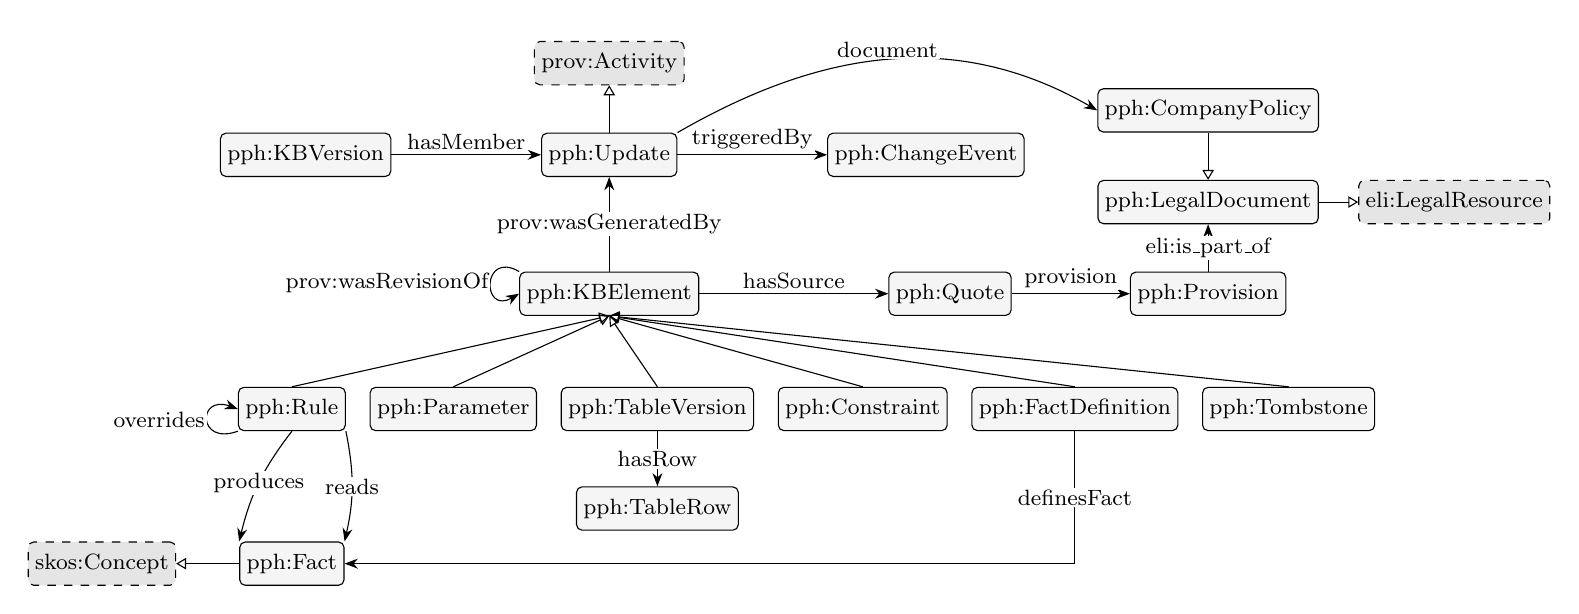
\begin{tikzpicture}[
  node distance=6mm and 7mm,
  cls/.style={draw,rounded corners=2pt,fill=gray!8,font=\footnotesize,minimum height=5.5mm,inner sep=2.5pt},
  ext/.style={cls,fill=gray!20,dashed},
  sub/.style={-{Triangle[open]},thin},
  rel/.style={-{Stealth},thin},
  lab/.style={font=\footnotesize,fill=white,inner sep=0.8pt}]

% knowledge base elements
\node[cls] (el) {pph:KBElement};
\node[cls,below left=9mm and 22mm of el] (rule) {pph:Rule};
\node[cls,right=3mm of rule] (par) {pph:Parameter};
\node[cls,right=3mm of par] (tab) {pph:TableVersion};
\node[cls,right=3mm of tab] (con) {pph:Constraint};
\node[cls,right=3mm of con] (fd) {pph:FactDefinition};
\node[cls,right=3mm of fd] (tomb) {pph:Tombstone};
\foreach \n in {rule,par,tab,con,fd,tomb} \draw[sub] (\n.north) -- (el.south);
\node[cls,below=7mm of tab] (row) {pph:TableRow};
\draw[rel] (tab) -- node[lab]{hasRow} (row);

% facts
\node[cls,below=14mm of rule] (fact) {pph:Fact};
\node[ext,left=8mm of fact] (concept) {skos:Concept};
\draw[sub] (fact) -- (concept);
\draw[rel] (rule.south) to[bend right=12] node[lab]{produces} (fact.north west);
\draw[rel] (rule.south east) to[bend left=12] node[lab]{reads} (fact.north east);
\draw[rel] (fd.south) |- node[lab,pos=0.25]{definesFact} (fact.east);
\draw[rel] (rule.south west) to[out=200,in=160,looseness=5] node[lab,left]{overrides} (rule.west);

% provenance
\node[cls,right=24mm of el] (quote) {pph:Quote};
\node[cls,right=15mm of quote] (prov) {pph:Provision};
\node[cls,above=6mm of prov] (doc) {pph:LegalDocument};
\node[ext,right=5mm of doc] (eli) {eli:LegalResource};
\node[cls,above=6mm of doc] (pol) {pph:CompanyPolicy};
\draw[rel] (el) -- node[lab,above=1pt]{hasSource} (quote);
\draw[rel] (quote) -- node[lab,above=1pt]{provision} (prov);
\draw[rel] (prov) -- node[lab]{eli:is\_part\_of} (doc);
\draw[sub] (doc) -- (eli);
\draw[sub] (pol) -- (doc);

% changes and versions
\node[cls,above=12mm of el] (upd) {pph:Update};
\node[cls,left=19mm of upd] (ver) {pph:KBVersion};
\node[cls,right=19mm of upd] (ev) {pph:ChangeEvent};
\node[ext,above=6mm of upd] (act) {prov:Activity};
\draw[rel] (el) -- node[lab]{prov:wasGeneratedBy} (upd);
\draw[rel] (ver) -- node[lab,above=1pt]{hasMember} (upd);
\draw[rel] (upd) -- node[lab,above=1pt]{triggeredBy} (ev);
\draw[sub] (upd) -- (act);
\draw[rel] (upd.north east) to[out=30,in=150] node[lab,above]{document} (pol.west);
\draw[rel] (el.north west) to[out=150,in=210,looseness=5] node[lab,left]{prov:wasRevisionOf} (el.west);

\end{tikzpicture}
}
\caption{Ontology of the knowledge base.}
\label{fig:ontology}
\end{figure*}

In the ontology of Fig.~\ref{fig:ontology}, classes reused from external vocabularies are drawn dashed. The two layers appear as a property of each rule, which also records its modality, its scope (period or year), its expression, and its condition.

Every rule belongs to one of two layers. Rules of the regulation layer state the law for all employers together with the conditions under which they apply, such as a list of business classification codes or a minimum number of workers. The engine checks these conditions against the profile of the company. Rules of the company layer belong to one policy of one company and may read any fact of the regulation layer. A rule also carries a modality (mandatory, default, or optional) with which the engine can let a company rule replace a default of the regulation while a mandatory provision always prevails. Calculation expressions are literal attributes of rules that the engine executes. A regulatory or policy change therefore touches only data in the graph. For example, the rounding rule of PER-11/PJ/2025 becomes a new version of the parameter \texttt{pph\_round\_mode} and not a change of code.

Every element records the interval in which it is legally valid and the date on which it was recorded. The two dates make the knowledge base bitemporal: a question asked on knowledge date $\omega$ sees only the regulation records with a recording date on or before $\omega$. Company records belong to the policies that a case names, and the engine reads the latest version of each.

An employer can compare the answers of two knowledge dates for the same month (Fig.~\ref{fig:bitemporal}). Employee B has status TK/0 and a monthly salary of Rp8,000,000 at an employer in a labor-intensive sector that is eligible under PMK 10/2025. The PPh 21 of this employee for January 2025 is Rp125,448. A question about January asked on 31 January returns no government-borne tax because PMK 10/2025 has not yet been issued. The same question asked on 10 February returns Rp125,448 borne by the government and paid to the employee in cash. Both answers stay available. Their difference is the correction that the employer owes for January. All values in the figure are engine output.

\begin{figure}[!t]
\centering
\figBitemporal
\caption{Two knowledge dates for the January 2025 tax of Employee B.}
\label{fig:bitemporal}
\end{figure}

\subsection{Inference Engine and Recalculation}
\label{sec:engine}
The engine computes the tax of one employee for a full tax year at a knowledge date $\omega$. It applies Algorithm~\ref{alg:engine} to every output fact of every period and then to the year facts of the final period. The algorithm works backward from the requested fact and stores each result, so an input is computed only once and only when a rule reads it. Conflicts between rules are resolved in the legal order of \emph{lex superior}, \emph{lex specialis}, and \emph{lex posterior}. Gross-up is computed as the least fixed point of the tax allowance because the allowance depends on the tax that it covers. A money value that is not a whole rupiah raises an error instead of being rounded silently because all arithmetic is exact.

\begin{algorithm}[!t]
\caption{Evaluation of one fact by the inference engine}
\label{alg:engine}
\footnotesize
\begin{algorithmic}[1]
\REQUIRE fact $f$, period or year $p$, knowledge date $\omega$, case data of one employee
\ENSURE value of $f$ in $p$ with its rule and quotes
\IF{a value of $f$ in $p$ is stored}
\RETURN the stored value
\ENDIF
\STATE $V \gets$ regulation records recorded on or before $\omega$ and the latest records of the policies that the case names
\STATE $A \gets$ rules in $V$ that produce $f$ and are valid in $p$, without optional regulation that the company has not adopted
\STATE remove from $A$ every rule whose condition does not hold in $p$
\IF{$A$ is empty}
\STATE raise an engine error
\ENDIF
\STATE keep in $A$ the rules of the highest rank (\emph{lex superior}: mandatory regulation, company rule, adopted optional regulation, default)
\STATE report a conflict for each company rule that lost to a mandatory rule with a different value
\STATE remove from $A$ every rule that another rule in $A$ overrides (\emph{lex specialis})
\STATE keep in $A$ the rules with the latest start of validity and then the latest recording (\emph{lex posterior})
\IF{the rules in $A$ give different values}
\STATE raise an engine error
\ENDIF
\STATE $r \gets$ the first rule in $A$
\STATE $v \gets$ the value of the expression of $r$, or its least fixed point for gross-up, where every fact that the expression reads is evaluated with this algorithm
\STATE check the type of $v$, store $v$ for $f$ in $p$, and record $r$ with its quotes
\RETURN $v$
\end{algorithmic}
\end{algorithm}

The calculator of the application shows the rule behind a result for a sample employee of Company C (Fig.~\ref{fig:calc}). The result card of the final month lists the values that the winning rule reads and names the rule with its provision, and the table beside it gives the withholding of every month.

\begin{figure*}[!t]
\centering
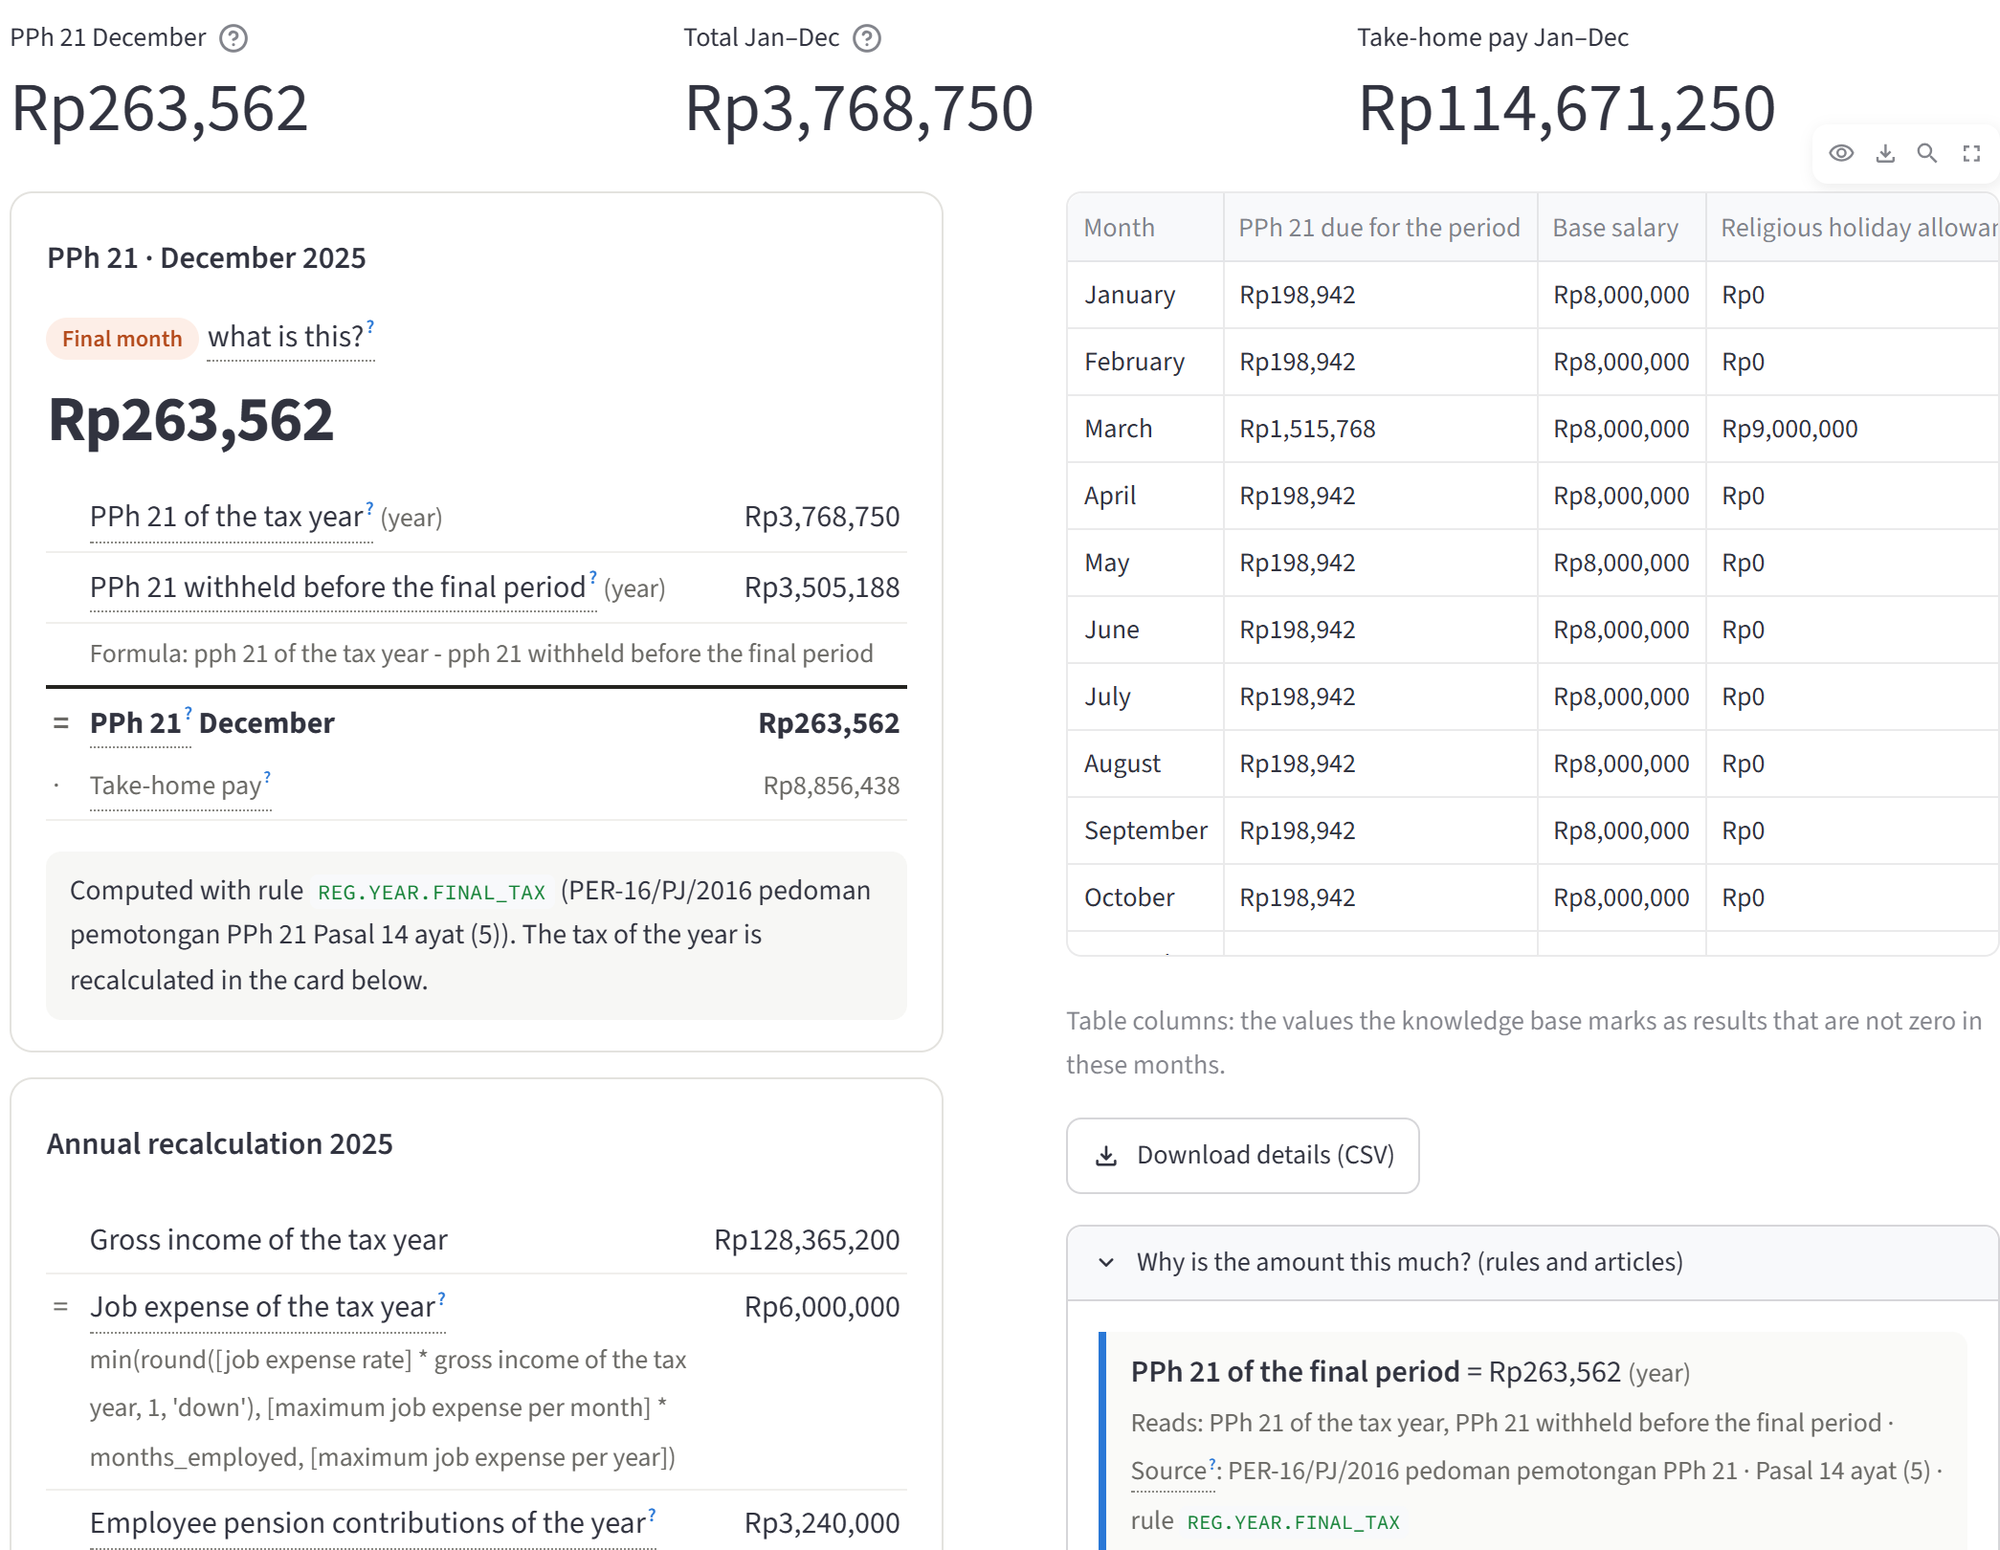
\includegraphics[width=0.9\textwidth]{figs/screen_calculator.png}
\caption{PPh 21 calculator of the application with the result of the final month and its rule.}
\label{fig:calc}
\end{figure*}

A retroactive rule needs no special code even when its update is recorded on date $\omega_1$ after a payroll has run on the knowledge of $\omega_0 < \omega_1$. The recalculation report then evaluates each employee at both knowledge dates and lists every value that differs in the months already paid. The employer receives the correction per employee and month. The payroll as computed on $\omega_0$ remains reproducible because no record is overwritten.

\subsection{LLM-Assisted Update Pipeline}
\label{sec:acquisition}
The update pipeline turns one document into at most one proposed update (Fig.~\ref{fig:acqflow}). It locks the document text with SHA-256 and splits it into parts by article. A low-cost model first maps each part as core (sent word for word), general (sent as a summary), or none (left out). Core parts are never cut. A drafting model then judges whether the document changes the PPh 21 computation and must support its judgment with verbatim quotes. A document judged not relevant ends with an empty update. For a relevant document, the drafting model writes three independent drafts of the update as structured JSON. Each draft lists the elements to add, change, or remove with a quote from the provision of each element. The prompt carries the vocabulary of facts and functions, the payroll data dictionary of the company, and the related records of the knowledge base retrieved with SPARQL. The model never computes tax.

\begin{figure*}[!t]
\centering
\figAcquisitionFlow
\caption{Update pipeline for one document.}
\label{fig:acqflow}
\end{figure*}

Six deterministic gates check every draft in the order of Table~\ref{tab:gates} and stop at the first failure. The static checks run first because G4 and G5 must execute the engine on generated cases. G6 is static and therefore runs second although it is numbered last. G1 applies the JSON schema, the application of the update to the knowledge base, and the SHACL shapes. G6 requires every case-data input that a new rule reads to exist in the payroll data of the company. Without this gate, a draft could invent an input such as an employee attribute that the generated test cases supply but real payroll data never contains. G2 requires each quote to occur in the document and every new number and date to occur in the quote of its element. G3 checks expressions, the dependency graph, and references. G4 runs the knowledge base before and after the update on a set $\SG$ of up to 300 cases generated from the draft and rejects new engine errors and changes before the start of validity.

The set $\SG$ combines PTKP statuses, withholding methods, salary levels, and the thresholds of the changed elements and is filled with random combinations to about 250 cases. It is generated from the draft alone and never reads the reference knowledge base or the test cases. G5 reports elements that change no output on $\SG$ to the reviewer without rejecting the draft. A draft that fails receives the gate messages and one repair round. Among the 354 drafts of the isolated runs, 151 failed a gate at first, and 31 of them passed after the repair round. A completeness gate G7 was defined after the evaluation and is reported separately in Section~\ref{sec:res-gate}.

\begin{table}[!t]
\caption{Verification gates and the first gate that failed among the 354 drafts of the isolated runs.}
\label{tab:gates}
\centering\footnotesize
\setlength{\tabcolsep}{3pt}
\begin{tabularx}{\columnwidth}{@{}lLLr@{}}
\toprule
Gate & Checks & Example of a failure & Drafts \\
\midrule
G1 & schema, application, SHACL & a missing required validity date or an annex table that was not extracted & 39 \\
G6 & inputs exist in payroll data & a rule reading an invented attribute for head-office staff & 96 \\
G2 & quotes, numbers, dates & an end of validity that no quote supports & 9 \\
G3 & expressions, references & a rule reading a table that is not yet valid & 2 \\
G4 & regression on $\SG$ & a tax facility that changes months before its start of validity & 5 \\
G5 & effect of each element & reported to the reviewer & 0 \\
\bottomrule
\end{tabularx}
\end{table}

The drafts that pass are grouped by their behavior on the union of their $\SG$ sets at the day before and the day of issue. Two drafts belong to the same group when they give the same output values, conflict report, and engine errors on every case of this union at both dates. The first draft of the largest group in a random order becomes the proposal. A single passing draft forms the largest group on its own. A tie or the absence of a passing draft ends in abstention, which sends the document to the HC software engineer without a proposal.

\subsection{Review by an HC Software Engineer}
\label{sec:review}
The intended reviewer is an HC software engineer of the human capital division. This engineer builds and maintains the company's human capital information system (HCIS) with its payroll module and can therefore read both the payroll data and the rules. The role exists in companies that develop their own HCIS. The review page shows the proposal with its quotes, the gate results, before-and-after payslips for a fixed set of payroll scenarios, and the company policies whose rules read a fact that the update touches. The engineer approves, edits, or rejects the proposal or asks the model to repair it. After an abstention the engineer writes the update. In both cases the engineer handles a structured change with its sources instead of writing new program code.

The application covers the upload of a document and the review of its proposal (Fig.~\ref{fig:manage}). A document is uploaded with its title, issue date, and type and waits on its card until the update pipeline is run. The review page lists the proposed changes with their quotes, the gate results, and the before-and-after results of the standard scenarios. The proposal in the figure was written by hand for illustration. The checks on this proposal report that its source document is not in the knowledge base.

\begin{figure*}[!t]
\centering
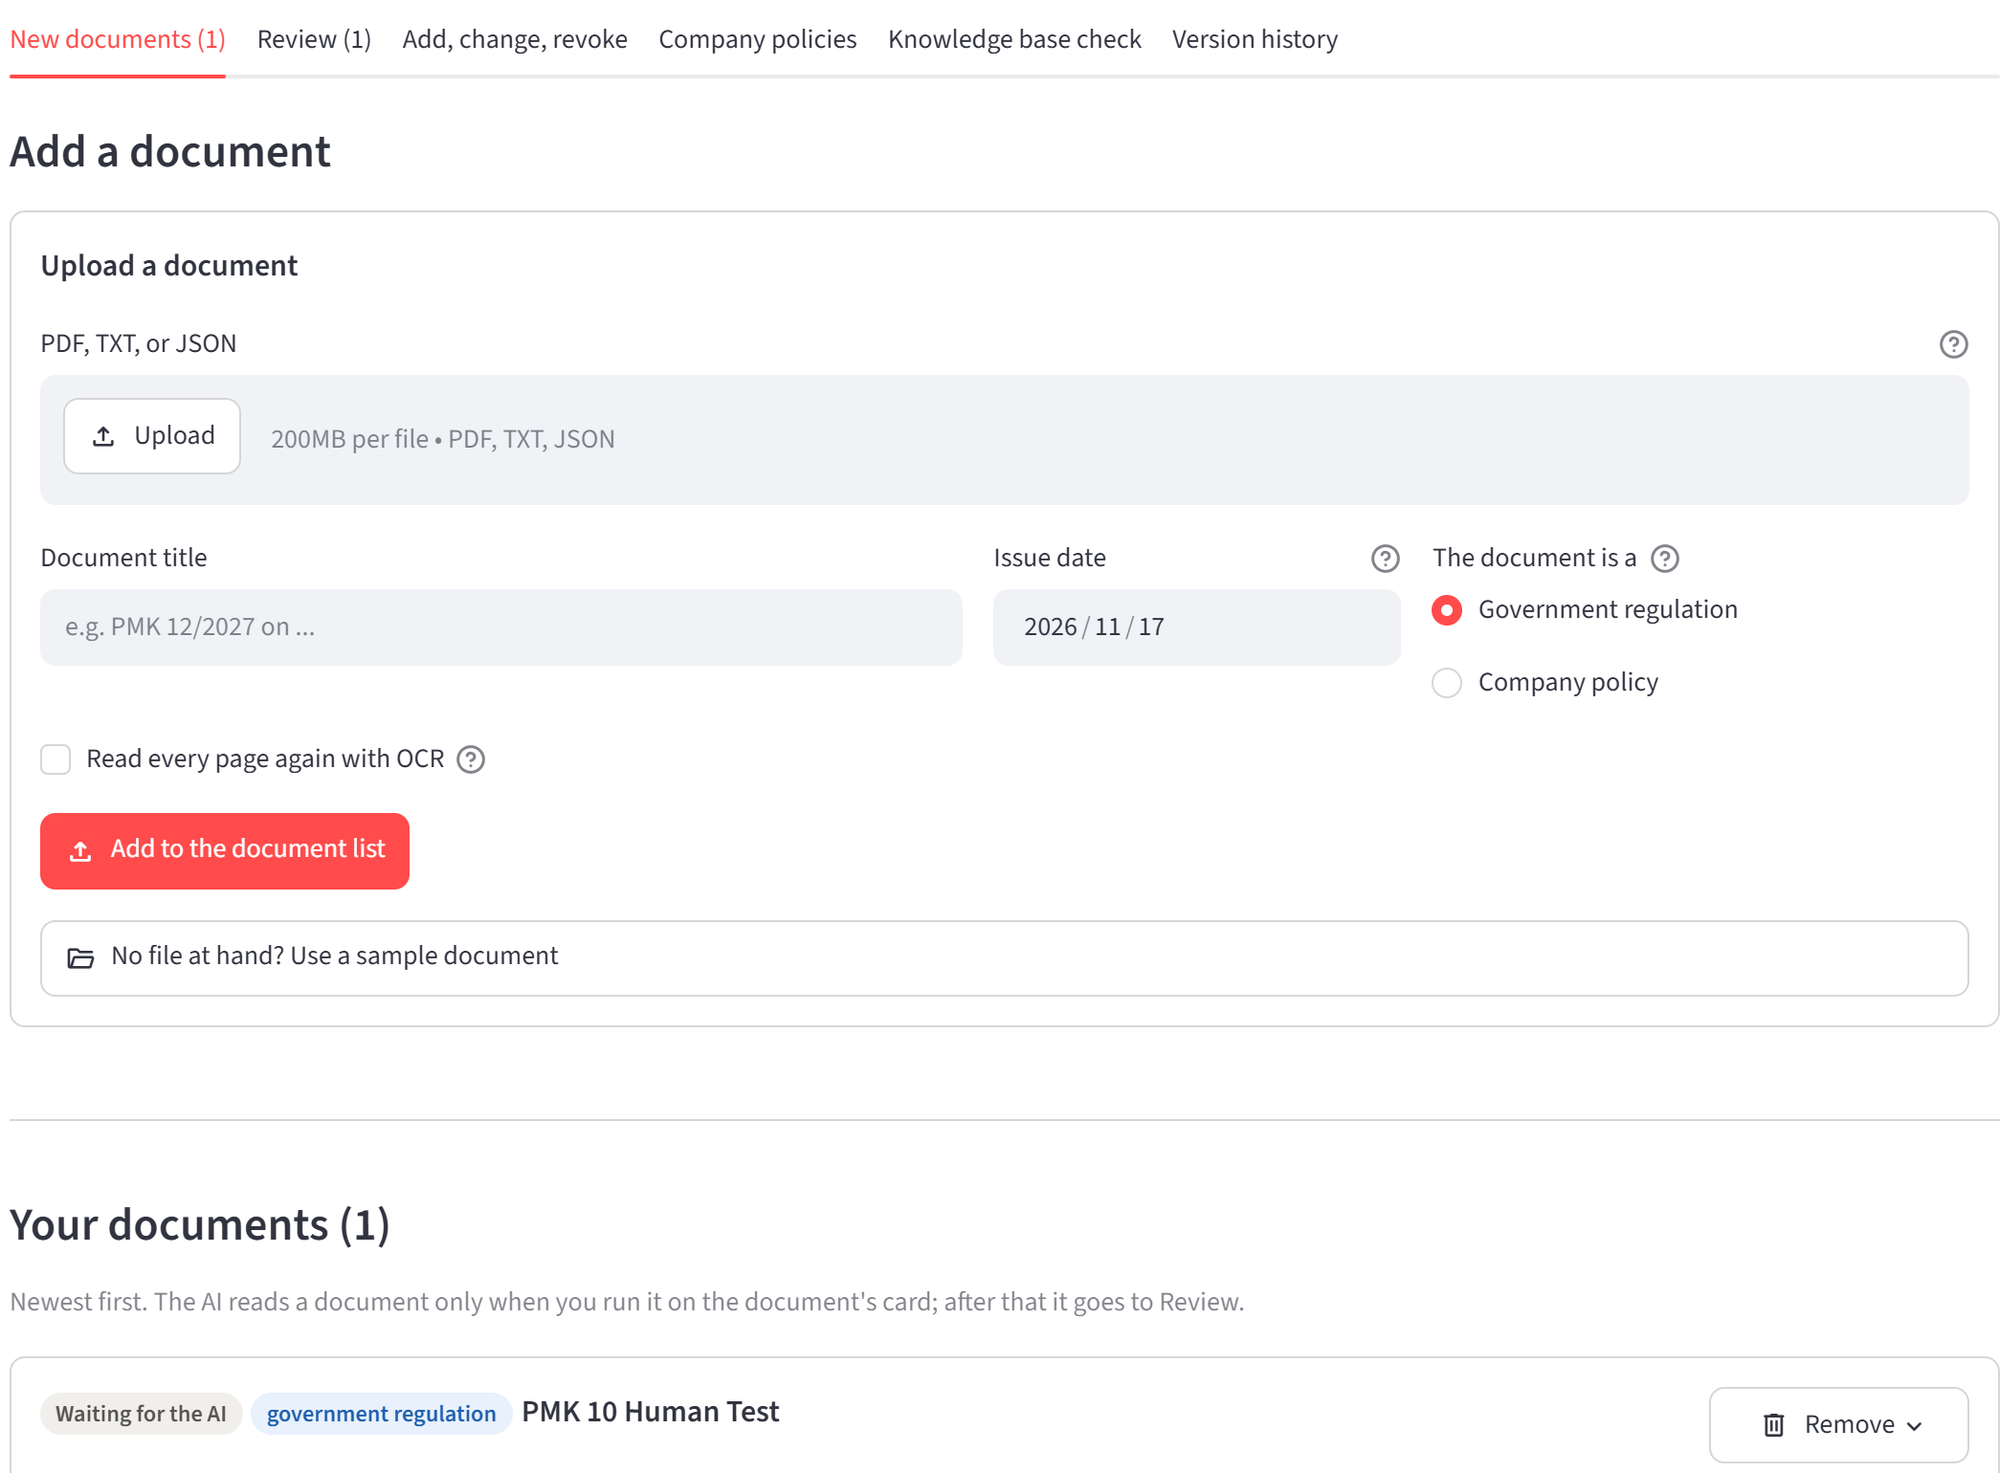
\includegraphics[width=0.6\textwidth]{figs/screen_upload.png}\\[1pt]{\footnotesize (a)}\\[4pt]
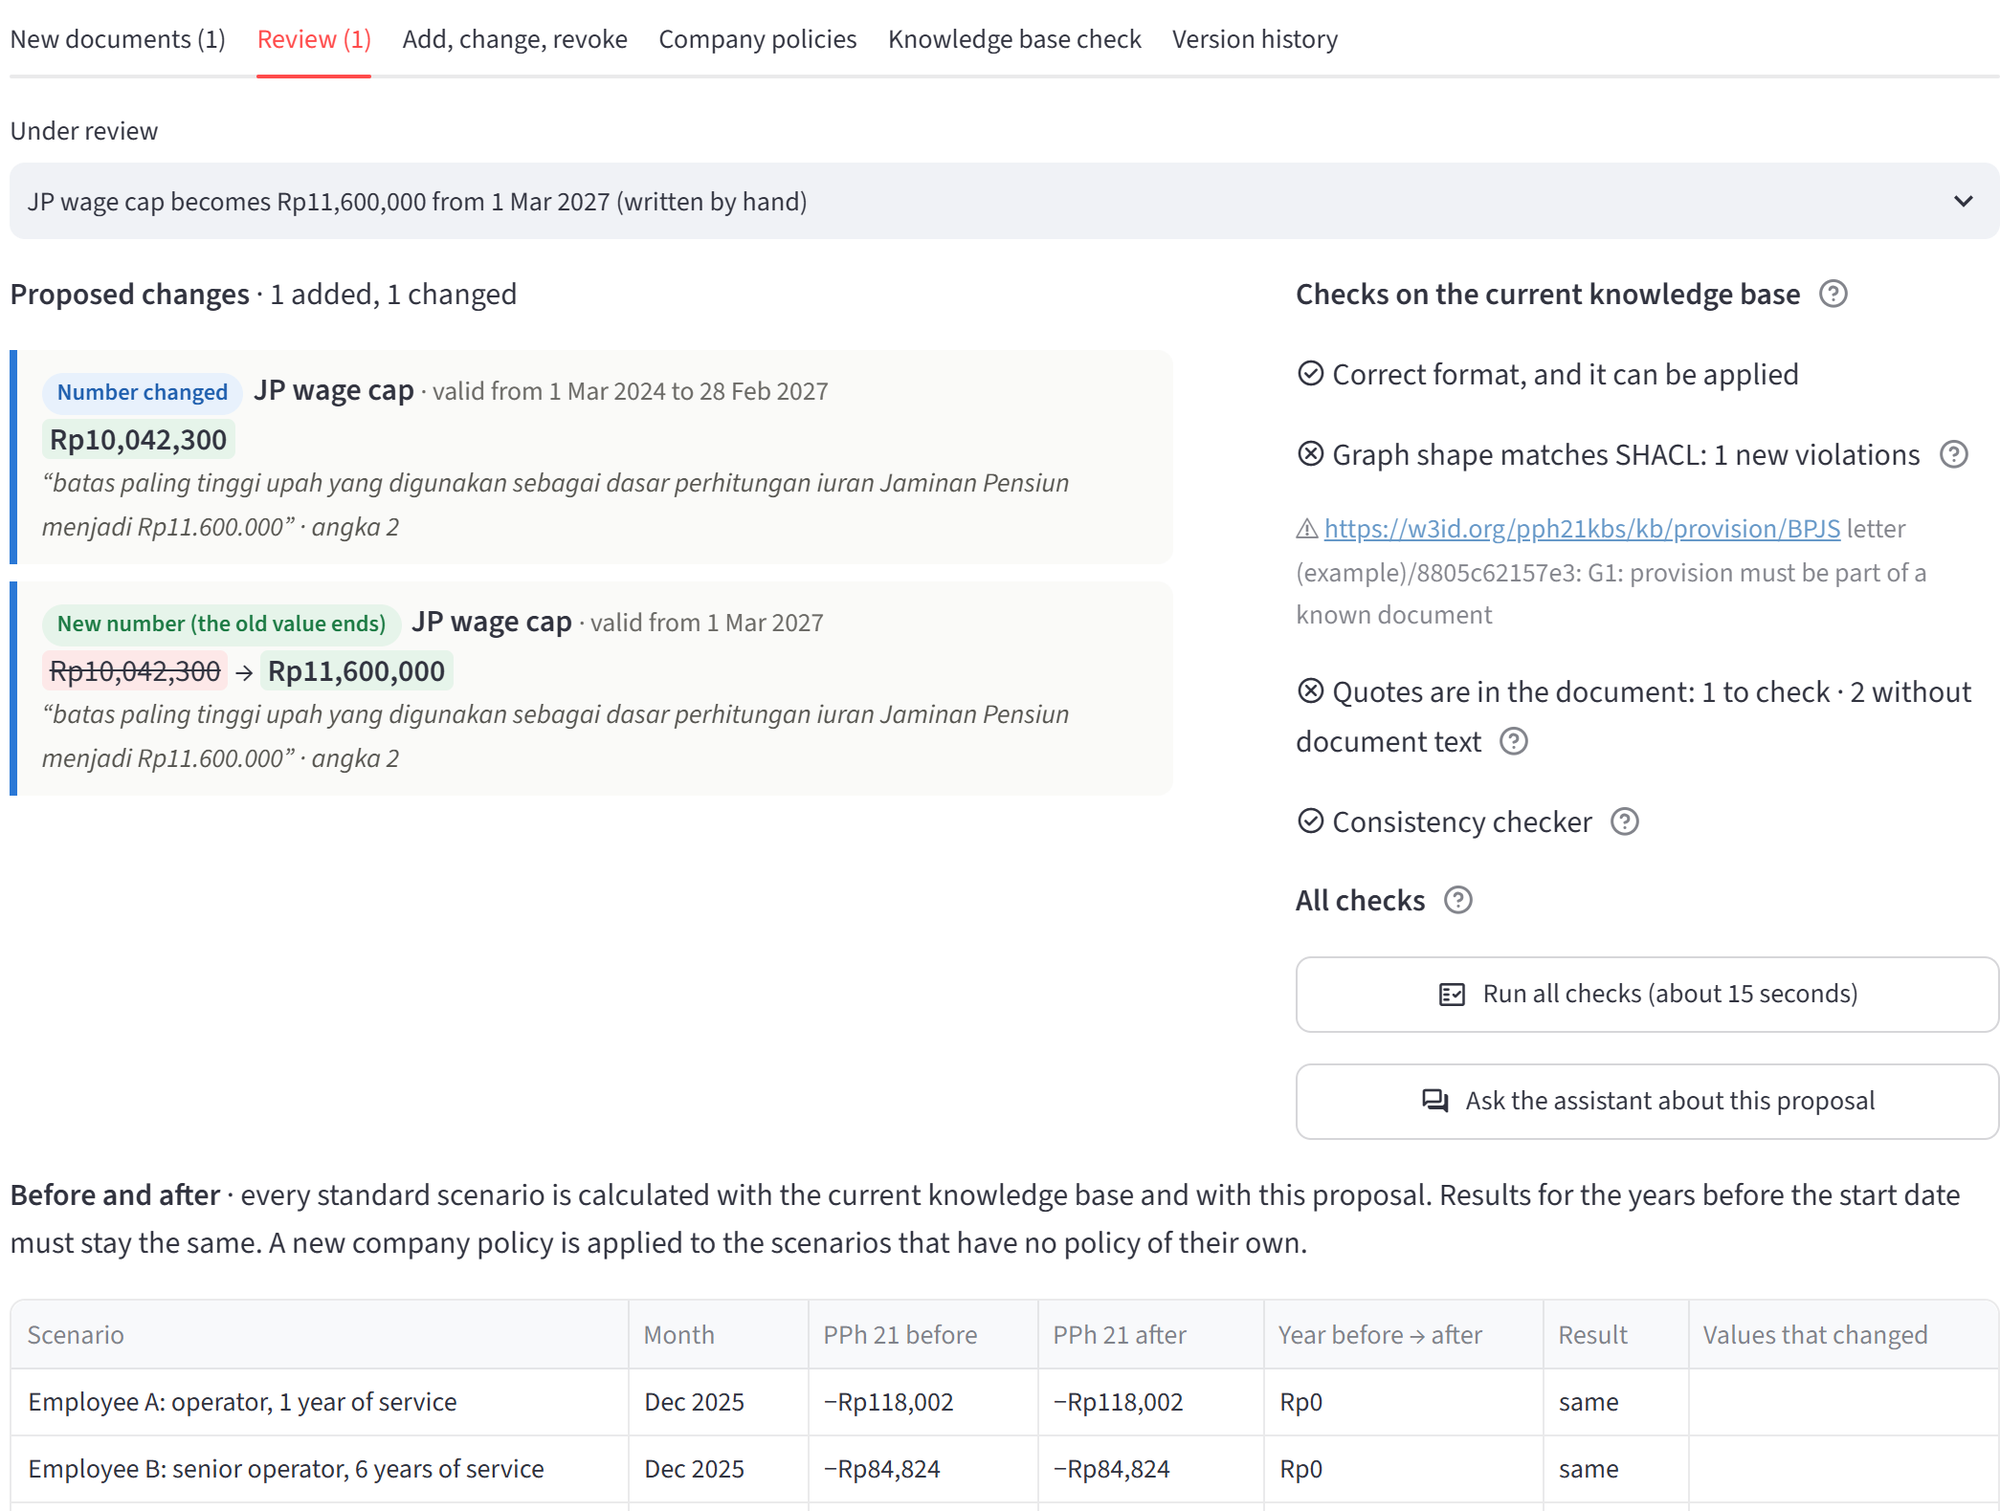
\includegraphics[width=0.6\textwidth]{figs/screen_review.png}\\[1pt]{\footnotesize (b)}
\caption{Knowledge base management with (a) the upload of a document and (b) the review of a proposal.}
\label{fig:manage}
\end{figure*}

% ============================================================================
\section{Evaluation Design}
\label{sec:design}
% ============================================================================
The evaluation follows how the system is used: one company installs one system and uploads every document it receives in the order of issue. It measures whether the representation recalculates past months correctly when a retroactive rule arrives (Section~\ref{sec:res-retro}) and how often a single drafted update is correct, silently wrong, or replaced by an abstention (Section~\ref{sec:res-single}). Its third measure is the share of a company's payslips that stay correct while the system's own updates accumulate, compared with a code-based update (Section~\ref{sec:res-chain}).

\subsection{Data}
\label{sec:data}
The test regulations are the 13 events of 2023--2026 that changed PPh 21 for permanent employees, five of them retroactive (Tables~\ref{tab:events} and~\ref{tab:data}). Twenty distractors are real regulations of the same period that do not change this computation, such as rules on other taxes. They stand for documents that a staff member uploads by mistake. Each was trimmed mechanically to its opening, the one article with the most PPh 21 terms, and its closing.

The five real companies have public collective labor agreements and come from five sectors and four provinces. This study refers to them as Companies A to E (Table~\ref{tab:data}). The scores of a company evaluate the proposed system on its public agreement and not the payroll that the company runs. Each company starts at its installation date, which is the signing date of its agreement or 1 January 2023 for an agreement signed earlier. Company B replaces its 2021 agreement with a new one in March 2024. Payslips are counted as employee-months scored in the chained mode. Ten fictional companies with synthetic policies cover combinations of business classification, workforce size, and work-accident risk group that the real companies do not.

\begin{table*}[!t]
\caption{The 13 test regulations of 2023--2026.}
\label{tab:events}
\centering\footnotesize
\setlength{\tabcolsep}{4pt}
\begin{tabularx}{\textwidth}{@{}llLll@{}}
\toprule
Event & Document & Change & Issued & Valid from \\
\midrule
E01 & BPJS letter B/77/022023 & pension wage cap 2023 & 2023-02-27 & 2023-03-01 \\
E02 & PMK 66/2023 & tax on benefits in kind & 2023-06-27 & 2023-07-01 \\
E03 & PP 58/2023 & TER withholding rates & 2023-12-27 & 2024-01-01 \\
E04 & PMK 168/2023 & implementing rules for TER & 2023-12-29 & 2024-01-01 \\
E05 & BPJS letter B/1387/022024 & pension wage cap 2024 & 2024-02-28 & 2024-03-01 \\
E06 & PMK 10/2025 & DTP, labor-intensive industry & 2025-02-04 & 2025-01-01 \\
E07 & PP 7/2025 & work-accident premium relief & 2025-02-07 & 2025-02-01 \\
E08 & BPJS letter B/726/022025 & pension wage cap 2025 & 2025-02-27 & 2025-03-01 \\
E09 & PP 36/2025 & extension of the premium relief & 2025-09-04 & 2025-08-01 \\
E10 & PMK 72/2025 & DTP extended to tourism & 2025-10-28 & 2025-10-01 \\
E11 & PMK 105/2025 & DTP for 2026 & 2025-12-31 & 2026-01-01 \\
E12 & BPJS letter B/1226/022026 & pension wage cap 2026 & 2026-02-25 & 2026-03-01 \\
E13 & PER-11/PJ/2025 & rounding to the nearest rupiah & 2025-05-22 & 2025-01-01 \\
\bottomrule
\end{tabularx}
\end{table*}

\begin{table}[!t]
\caption{Documents, companies, payslips, and reference rows of the evaluation.}
\label{tab:data}
\centering\footnotesize
\setlength{\tabcolsep}{3pt}
\begin{tabularx}{\columnwidth}{@{}lLr@{}}
\toprule
Item & Content & Count \\
\midrule
Test regulations & PPh 21 changes of 2023--2026, five retroactive & 13 \\
Distractors & real regulations that do not change PPh 21 & 20 \\
Real companies & Company A (garment), B (textile), C (footwear), D (aviation services), and E (construction) & 5 \\
Labor agreements & public agreements of the five companies & 6 \\
Fictional companies & synthetic policies, two simulation chains & 10 \\
Prospective units & unseen changes: 50 regulations, 30 company policies & 80 \\
Chain steps & documents processed in the seven chains & 224 \\
Payslips, real & employee-months of the five real companies & 26,328 \\
Payslips, simulation & employee-months of the fictional companies & 66,374 \\
Reference check & payslip rows checked by a tax practitioner & 262 \\
\bottomrule
\end{tabularx}
\end{table}

Thirteen real changes are too few for statistical tests of single updates, so a prospective set adds 80 test units. Each unit describes a change that has not happened but could, such as a new PTKP amount, a new TER table, a new DTP sector, a new pension wage cap, or a new gross-up policy. Each unit follows the format of its source document type (letterhead, considerations, articles, annex tables) and passes through PDF rendering and the same extraction pipeline as the real documents. Traps such as a cross-reference, an exception, a transitional provision, or a number found only in an annex appear at least once in every unit. A mechanical check confirmed for each unit that its reference update passes the gates, that every quote is found in the extracted text, and that it changes at least one payslip. The units were written with a model from a different family than the drafting model.

Each company has a panel of about 150 active employees per year in 2023--2026, including joiners and leavers. Their wages are drawn from the wage cells of Statistics Indonesia for the company's sector and province. Their pay components follow the company's labor agreement. Employees at, just below, and just above every threshold that a change touches are added so that every change reaches at least one payslip.

\subsection{Reference Knowledge Base}
\label{sec:reference}
Every test document was encoded by hand in a reference knowledge base from which the engine computes every reference payslip. A tax practitioner checked the reference calculations row by row in a workbook organized by criterion. The workbook covers monthly withholding under TER (113 rows), the 2023 annualized method (39 rows), tax borne by the employer (59 rows), and final-period recomputations (20 rows). It also holds 21 examples from the clauses of the five labor agreements and 10 further employee-months. The practitioner confirmed all 262 rows without correction. The checked cases span the tax years 2023 to 2026 and include benefits in kind, the pension wage cap, DTP with its tourism extension, the work-accident premium relief, and the rounding rule.

Before the measured runs, the engine and the reference knowledge base were also compared with two external sources. They matched 665 of 679 values in 26 worked examples published in the regulations, and every difference was an error in the published example. On 10 held-out examples they matched 221 of 235 values at the first comparison and 232 after the reference was corrected. The three remaining differences concern the mapping of a pension contribution and the rounding of half a rupiah. The official PPh 21 calculator of the tax authority gave the same tax in 15 of 20 monthly cases and the same 90 values in 15 final-period cases. Each of the five monthly differences is Rp1 because the calculator drops fractions, whereas PER-11/PJ/2025 requires rounding to the nearest rupiah.

\subsection{Evaluation Modes}
\label{sec:modes}
The evaluation has two main modes (Fig.~\ref{fig:protocol}). The isolated mode applies each document to the reference knowledge base as it stood just before the document and scores the drafted update on its own. The 13 real regulations were run twice in this mode. In the chained mode, each real company has its own independent chain that starts from the reference knowledge base on its installation date and receives the company's documents in the order of issue. Every update that the system makes stays in the knowledge base that the next document meets, so an error can carry forward. The figure marks a regulation with E and a distractor with D. It denotes the reference knowledge base by $\K^\star$, a drafted update by $\hat\Delta$, the scored result by $\K'$, and the system's own knowledge base by $\K^{\mathrm{sys}}$. The ten fictional companies share two further chains as a simulation, in which each regulation is drafted once for five companies as a provider of the regulation layer would do.

\begin{figure*}[!t]
\centering
\figReplayProtocol
\caption{Isolated and chained evaluation modes.}
\label{fig:protocol}
\end{figure*}

A third mode tests late uploads. For each of the five retroactive events, the update drafted in the isolated mode is recorded one, two, and three months after the issue date when payrolls have already run. The recalculation report of the system is compared with that of the reference update recorded on the same day. The payroll as known before the upload is also checked to be unchanged.

\subsection{Reviewer Conditions and the Code-Based Update}
\label{sec:conditions}
Three reviewer conditions reuse the results of the single model run of each chain. In the \emph{reviewer} condition, the HC software engineer approves every proposal as it is and writes the reference update 26 days after issue whenever the system abstains. Approving every proposal is the worst case for silent errors because a wrong proposal looks like any other. The \emph{careful-reviewer} condition also rejects a proposal whose review payslips differ from those of the reference update and writes the update 26 days after issue instead. This condition assumes that every error visible on the review page is noticed. The condition \emph{without reviewer} leaves the knowledge base unchanged after an abstention and gives a lower bound for full automation.

The comparison is a \emph{code-based update} (baseline B1) that applies the correct update with the recalculation of past months 26 days after each issue. Twenty-six days is the fastest adoption of TER by an open-source PPh 21 calculator in its commit history. The other calculator took 915 days. The code-based update is therefore a favorable stand-in for current practice because it is always correct and only late. Its disadvantage is limited to the payslips whose payroll date falls within 26 days after an issue. The system is assumed to apply an approved update on the issue date.

\subsection{Baselines for a Single Update}
Three baselines use the same drafts as the system and differ only in how a draft is chosen. B2 takes the first draft in the random order that passes all gates, without consensus or abstention. B3 takes the first draft that passes the schema and quote checks before repair. B4 takes the behavioral majority of all drafts without gates, as in the closest work~\cite{goganikhiabani2025maintaining}. An upper bound counts a document as correct when any passing draft is correct.

\subsection{Metrics and Statistics}
\label{sec:metrics}
A single update is \emph{correct} when every output value, the conflict report, and the engine errors equal those of the reference update on every test case. The comparison is made on the day before the document was issued and on the day of issue. The test cases are the employee-years of the affected tax years in a fixed test space that is separate from $\SG$. One value off by one rupiah makes the update a \emph{silent error}. Abstentions are reported separately. The silent-error rate (SER) is the share of documents with a silent error.

Payslip accuracy is the share of employee-months whose payslip equals the reference payslip to the rupiah in every output of the engine, such as gross income, PPh 21 withheld, government-borne tax, and take-home pay. Each payslip is scored twice: as known on the payroll date of its month (the 25th) and as known at the end of the test window after every retroactive rule has been applied. The first score measures what the employee was paid. The second measures whether the company ends with correct books.

Rates carry Clopper--Pearson intervals~\cite{clopper1934use}. The system and B3 are compared with the exact McNemar test~\cite{mcnemar1947note} and a Newcombe interval for paired proportions~\cite{newcombe1998improved}. The difference in payslip accuracy between the system and the code-based update carries a 95\% bootstrap interval with 10,000 resamples over the 54 event--chain pairs of the real companies~\cite{field2007bootstrapping}. These pairs are the resampling clusters because the payslips that one event affects are not independent. Agreement between drafting models uses Cohen's kappa~\cite{cohen1960coefficient}.

\subsection{Hypotheses and Procedure}
Two hypotheses and their thresholds were fixed in an analysis plan before the measured runs. H1 states that payslip accuracy on the payroll date in the reviewer condition is not lower than that of the code-based update by more than 0.01. Its test requires the lower bound of the 95\% interval of the difference to lie above $-0.01$. H1 also states that no error propagates systematically: no event may be correct in both isolated runs but wrong in at least two chains. H1 is reported as an estimate with its interval because a power simulation from the development runs gave 0.64, below the planned 0.80. H2 concerns single updates on the prospective set: a one-sided 95\% upper bound of SER of at most 0.15, a lower SER than B3, and an abstention rate of at most 0.50.

The system drafts with \texttt{gpt-6.1-sol} at high reasoning effort and maps documents with \texttt{gpt-5.4-mini}. Each drafting prompt holds the vocabulary of the knowledge base, up to 220 of its records that relate to the document, the payroll attributes of the company, and the document text. The model answers in a fixed JSON schema with at most 32,000 output tokens per call, and the relevance judgment uses medium reasoning effort. The prompts are part of the released code. Claude Sonnet 5.5 repeats the real set as a robustness check. The system was frozen after prompts and gates had been tuned only on development data, namely the events of 2012--2022 and four synthetic policies. Every number in Section~\ref{sec:results} can be recomputed from the logs without calling a model because every model call of the measured runs was logged.

The analysis plan also listed a cross-layer impact analysis, a full-text reading of long documents, a baseline in which an LLM patches calculator code, and a timing study of the engineer. These analyses were not carried out within the budget of the study. One relevance call in the chain of Company E timed out. The system then drafted the distractor because it treats a timed-out relevance call as a judgment of relevance, as it does in operation. Runs interrupted by network failures were resumed from the logged model answers without changing them.

% ============================================================================
\section{Results}
\label{sec:results}
% ============================================================================
\subsection{Recalculation Under Retroactive Rules}
\label{sec:res-retro}
The payroll as known before the upload stayed unchanged in all 15 late-upload scenarios (Table~\ref{tab:late}), as the append-only records of the knowledge base guarantee. The employer can therefore still reproduce what was withheld at the time. The reference updates changed the paid withholding of 3,276 employee-months summed over the scenarios. The affected test cases ranged from one under the tourism extension of E10 to about 250 under the rounding rule of E13. Cases in the table are test employee-years whose paid withholding or annual values change under the reference update, and paid months are the changed months already paid. The report covered more months the longer the upload was delayed. No code was changed in any scenario.

\begin{table}[!t]
\caption{Late upload of the five retroactive rules.}
\label{tab:late}
\centering\footnotesize
\setlength{\tabcolsep}{3pt}
\begin{tabularx}{\columnwidth}{@{}lLrrc@{}}
\toprule
Event & Retroactive rule & Cases & Paid months, lag 1/2/3 & Report \\
\midrule
E06 & DTP for labor-intensive industry, 2025 & 24 & 20/21/35 & $\times\,\times\,\times$ \\
E07 & 50\% relief of the work-accident premium & 43 & 33/66/99 & \checkmark\,\checkmark\,\checkmark \\
E09 & extension of the premium relief & 34 & 68/102/136 & \checkmark\,\checkmark\,\checkmark \\
E10 & DTP extended to tourism & 1 & 1/2/3 & \checkmark\,\checkmark\,$\times$ \\
E13 & rounding to the nearest rupiah & 249--250 & 751/898/1,041 & \checkmark\,\checkmark\,\checkmark \\
\midrule
Sum & 15 scenarios (earlier payroll reproducible in all) & & 3,276 & 11 of 15 \\
\bottomrule
\end{tabularx}
\end{table}

The system's own recalculation report equaled the reference report in 11 of the 15 scenarios (report column of Table~\ref{tab:late}). All nine scenarios of the three events whose drafted update was correct (E07, E09, E13) matched exactly, among them the three scenarios of the rounding rule with up to 1,041 paid employee-months. The four differences came from the two updates that were already wrong in the isolated mode. The E06 update differed at every lag. The one wrong value of the E10 update fell in a month already paid only at the longest lag. The bitemporal representation thus turned a correct update into a correct retroactive correction at each of the three upload lags.

\subsection{Single Updates}
\label{sec:res-single}
In the isolated mode (Fig.~\ref{fig:outcomes}) the system made 41 correct updates and 15 silent errors (SER 0.19, one-sided upper bound 0.27) on the 80 prospective units and abstained on 24. Of the 39 updates proposed for regulation units, 35 were correct and 4 were silent errors. Parameter changes (T1) and changes of calculation method (T7) were correct in all 13 units of these types. Company-policy units were harder, with 6 of 30 correct, 13 abstentions, and 11 silent errors. Five of these 11 silent errors only named the amended policy differently from the reference. When the policy identifiers of memo updates were mapped to the policy in force, the prospective outcomes became 46 correct updates, 24 abstentions, and 10 silent errors.

The system drafted 9 of the 13 real regulations correctly and abstained on 2 of them and on all six labor agreements. A second run gave the same outcome for 12 of the 13 regulations. None of the 20 distractors changed a payslip: the system judged 13 of them not relevant, abstained on 5, and drafted updates without any effect for the other 2. Fig.~\ref{fig:outcomes} counts these 13 and 2 distractors as correct.

\begin{figure}[!t]
\centering
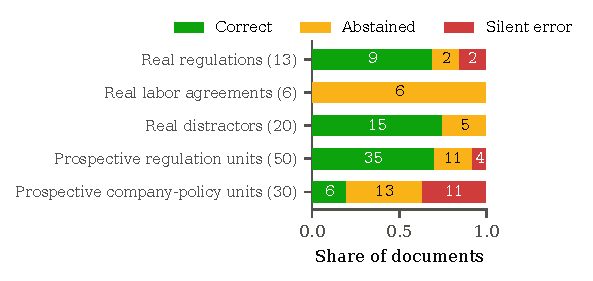
\includegraphics[width=\columnwidth]{figs/fig_outcomes.pdf}
\caption{Outcome of single updates in the isolated mode.}
\label{fig:outcomes}
\end{figure}

Among the baselines built from the same drafts (Table~\ref{tab:single}), the behavioral majority of all drafts without gates (B4) applied the selection rule of the closest work and made 24 silent errors on the prospective set and 2 on the real labor agreements. Every selection that used the gates made 13 to 15. The schema and quote checks alone (B3) already account for this reduction. The consensus did not add to it: the first draft that passes all gates (B2) was as accurate as the upper bound and made 43 correct updates against 41 for the system. The difference in correct updates between the system and B3 was $+0.025$ (95\% interval $-0.023$ to $0.072$). Each cell of Table~\ref{tab:single} gives correct updates, abstentions, and silent errors in this order.

\begin{table}[!t]
\caption{Single updates of the system and the baselines built from the same drafts.}
\label{tab:single}
\centering\footnotesize
\setlength{\tabcolsep}{3pt}
\begin{tabular}{@{}lccc@{}}
\toprule
Selection & Prospective & Regulations & Agreements \\
 & (80) & (13) & (6) \\
\midrule
System & 41 / 24 / 15 & 9 / 2 / 2 & 0 / 6 / 0 \\
B2, first passing draft & 43 / 23 / 14 & 10 / 2 / 1 & 0 / 6 / 0 \\
B3, first draft passing G1--G2 & 39 / 28 / 13 & 8 / 3 / 2 & 0 / 6 / 0 \\
B4, majority without gates & 41 / 15 / 24 & 10 / 2 / 1 & 0 / 4 / 2 \\
Upper bound & 43 / 23 / 14 & 10 / 2 / 1 & 0 / 6 / 0 \\
\bottomrule
\end{tabular}
\end{table}

Claude Sonnet 5.5 as drafting model gave 26 correct updates, 6 abstentions, and 7 silent errors on the 39 real documents, against 24, 13, and 2 for \texttt{gpt-6.1-sol}. The two models agreed on 29 of the 39 documents ($\kappa = 0.52$) and on 12 of 20 prospective units ($\kappa = 0.40$). Sonnet abstained less often and accepted two distractors as changes.

\subsection{Payslip Accuracy of Companies Over Time}
\label{sec:res-chain}
In the reviewer condition, payslip accuracy on the payroll date (Fig.~\ref{fig:payslip} and Table~\ref{tab:chain}) was 0.978 at Company A, 0.961 at Company B, 0.945 at Company C, and 1.000 at Company E. In each of these four companies the share of correct payslips exceeded that of the code-based update by about two to three percentage points. This margin arose because the system brought each correct regulation into the payroll on its issue date instead of 26 days later. This advantage is confined to the payslips whose payroll date falls within 26 days after an issue. Accuracy at Company D was 0.239, which Section~\ref{sec:res-gate} traces to a single proposal. Accuracy pooled over the five companies was 0.842 against 0.951 for the code-based update. The series with the completeness gate in Figs.~\ref{fig:payslip} and~\ref{fig:monthly} belong to the design iteration of Section~\ref{sec:res-gate}.

The code-based update and the reviewer condition lose payslips in different months (Fig.~\ref{fig:monthly}). At Companies A, B, and C the code-based update loses all or nearly all payslips of February and September 2025 and part of those of May 2025 and January 2026, the months whose payroll date falls within the 26 days after a change. The reviewer condition loses payslips mostly in December, when the year is recomputed. Company B also loses February 2025 in this condition because the engineer's update for E06 arrived after the payroll date. At Company D the reviewer condition loses every payslip from April 2024 to March 2026, whereas the completeness gate keeps Company D correct in every month.

\begin{figure*}[!t]
\centering
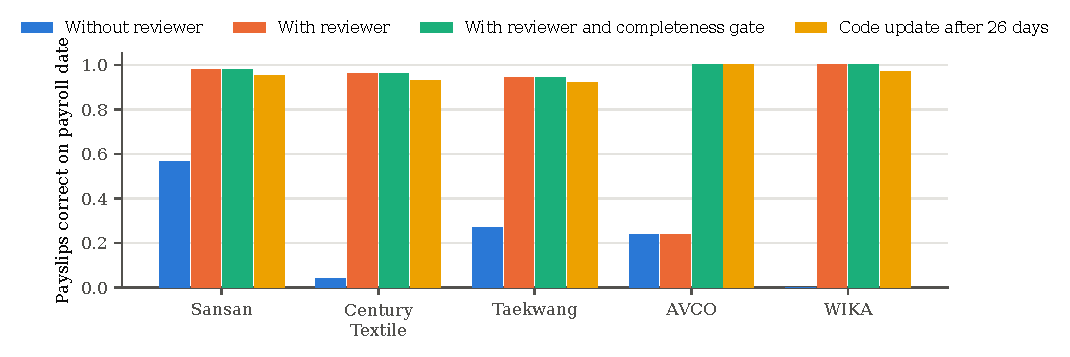
\includegraphics[width=0.92\textwidth]{figs/fig_payslip.pdf}
\caption{Payslip accuracy on the payroll date in the five real companies under each condition.}
\label{fig:payslip}
\end{figure*}

\begin{figure*}[!t]
\centering
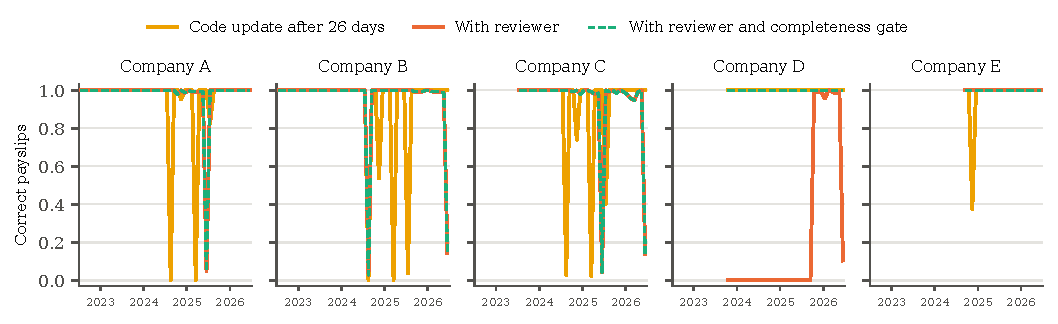
\includegraphics[width=0.95\textwidth]{figs/fig_monthly.pdf}
\caption{Monthly payslip accuracy on the payroll date in the five real companies.}
\label{fig:monthly}
\end{figure*}

\begin{table*}[!t]
\caption{Payslips, documents, engineer-written updates, accuracy, and cost of the chained mode.}
\label{tab:chain}
\centering\footnotesize
\setlength{\tabcolsep}{3pt}
\resizebox{\textwidth}{!}{%
\begin{tabular}{@{}lrrrrrrrrrrr@{}}
\toprule
 & & & Written by & \multicolumn{4}{c}{Accuracy on the payroll date} & \multicolumn{3}{c}{Accuracy at the end of the window} & \\
\cmidrule(lr){5-8}\cmidrule(lr){9-11}
Company & Payslips & Documents & engineer & Without reviewer & Reviewer & Careful reviewer & Code-based & Reviewer & Careful reviewer & Code-based & Cost (USD) \\
\midrule
Company A & 7,026 & 34 & 3 & 0.566 & 0.978 & 0.994 & 0.953 & 0.978 & 1.000 & 1.000 & 8.57 \\
Company B & 6,747 & 35 & 5 & 0.041 & 0.961 & 0.954 & 0.930 & 0.981 & 0.986 & 1.000 & 9.64 \\
Company C & 5,039 & 27 & 1 & 0.268 & 0.945 & 0.967 & 0.922 & 0.945 & 1.000 & 1.000 & 4.68 \\
Company D & 4,558 & 25 & 0 & 0.239 & 0.239 & 0.239 & 1.000 & 0.239 & 0.239 & 1.000 & 4.39 \\
Company E & 2,958 & 17 & 2 & 0.000 & 1.000 & 1.000 & 0.969 & 1.000 & 1.000 & 1.000 & 3.83 \\
\midrule
Real companies, pooled & 26,328 & 138 & 11 & 0.254 & 0.842 & 0.849 & 0.951 & 0.847 & 0.865 & 1.000 & 31.11 \\
\midrule
Simulation A (5 companies) & 33,175 & 43 & 6 & 0.651 & 0.911 & 0.942 & 0.986 & 0.911 & 0.939 & 1.000 & 9.87 \\
Simulation B (5 companies) & 33,199 & 43 & 4 & 0.844 & 0.824 & 0.958 & 0.993 & 0.824 & 0.958 & 1.000 & 8.46 \\
\bottomrule
\end{tabular}}
\end{table*}

The end of the window shows the cost of the silent errors. The code-based update is correct by construction once it arrives and reached 1.000 everywhere, whereas the system kept the effect of its silent errors and ended at 0.945 to 1.000 in the four companies. The careful-reviewer condition raised the end-of-window accuracy to 1.000 at Companies A and C by rejecting each proposal whose review payslips differ from those of the reference update. At Company B it scored lower on the payroll date than the reviewer condition (0.954 against 0.961) because each rejected proposal is replaced by an update written 26 days after issue.

The engineer wrote the update by hand for 11 of the 138 documents that the five companies received (Fig.~\ref{fig:workload}), each time after an abstention. The other 14 abstentions concerned documents without effect on the payroll. The figure also counts the 59 documents judged not relevant and the 11 proposals without effect on any payslip. The system decided the remaining 113 documents at a model cost of about USD 0.23 per document. The 54 steps that carried a real change comprised 33 correct proposals, 11 updates written by the engineer, and 10 silently wrong proposals that the reviewer condition approved. The labor agreements that install the company layer were the weak point: the engineer wrote five of the six, and the sixth was the incomplete proposal for Company D. These abstained installations also explain the low accuracy without a reviewer (0.000 at Company E and 0.041 at Company B) because the company layer then stays empty.

\begin{figure*}[!t]
\centering
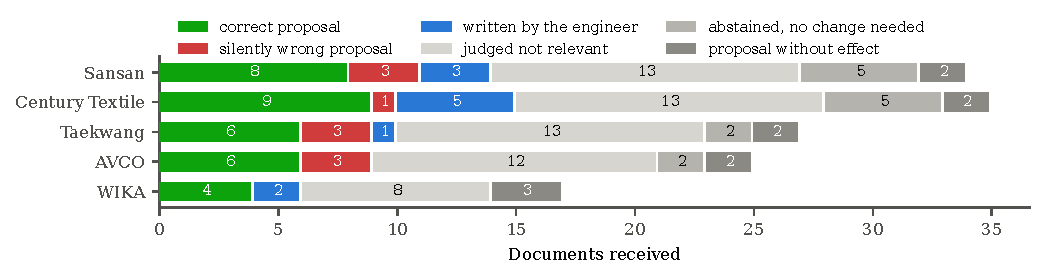
\includegraphics[width=0.92\textwidth]{figs/fig_workload.pdf}
\caption{Decision on each document received by the five real companies.}
\label{fig:workload}
\end{figure*}

The simulation chains confirm that unchecked company-policy proposals carry the most risk. Their fictional companies received synthetic policy memos, the type of document that was hardest in the isolated mode. Both chains stayed below the code-based update in the reviewer condition. In Simulation B approving every proposal (0.824) was worse than leaving every abstention unhandled (0.844). The careful-reviewer condition recovered most of the gap in Simulation B and about two fifths of it in Simulation A.

\subsection{Error Propagation and Pre-Specified Hypotheses}
\label{sec:res-hyp}
In 40 of the 48 pairs of a regulation and a real company, the update in the chain had the same outcome as the first isolated run of the same regulation. Four pairs improved in the chain, where a silent error of the isolated run became a correct update or an abstention. The 2026 DTP regulation (E11) went the other way: it was correct in both isolated runs but wrong in four of the five chains. E11 extends the facility rules of E06 and E10. In the chains it was drafted against the system's own knowledge base, whose earlier updates differed from the reference. Which difference triggered the error was not isolated. The labor agreement of Company D adds a ninth discrepancy because the system abstained on it in isolation but proposed an update in its chain.

H1 is not supported (Table~\ref{tab:hyp}). The reviewer condition differed from the code-based update by $-0.109$ pooled over the five real companies (95\% interval $-0.345$ to $0.030$ over 54 event--chain clusters). This result was driven by Company D, without which the difference was $+0.027$. E11 also meets the pre-specified definition of systematic propagation.

On the prospective set the SER of 0.19 exceeded its threshold of 0.15, and the system made 15 silent errors against 13 for B3. H2 is therefore not supported either, although the abstention rate of 0.30 met its threshold.

\begin{table}[!t]
\caption{Pre-specified hypotheses and their outcomes.}
\label{tab:hyp}
\centering\footnotesize
\setlength{\tabcolsep}{3pt}
\begin{tabularx}{\columnwidth}{@{}Lll@{}}
\toprule
Criterion & Threshold & Result \\
\midrule
H1(a) accuracy vs code-based update & bound $> -0.01$ & $-0.109$ [$-0.345$, $0.030$] \\
H1(b) systematic propagation & none & E11 \\
H2(a) SER, prospective set & bound $\leq 0.15$ & 0.19 (bound 0.27) \\
H2(b) SER lower than B3 & McNemar $p < 0.05$ & 15 vs 13, $p = 0.89$ \\
H2(c) abstention rate & $\leq 0.50$ & 0.30 \\
\bottomrule
\end{tabularx}
\end{table}

\subsection{Design Iteration: A Completeness Gate}
\label{sec:res-gate}
The chain of Company D starts with the installation of its labor agreement. The proposal for this document declared two facts (a base salary and a radiation allowance) and added no rule that used them. The draft's own note stated that the update was not computationally complete. Such a proposal passes every gate because G5 checks the effect of rules and skips facts. Without any effect, the proposal also shows no difference on the review page. Payslip accuracy at Company D stayed at 0.239 until the end of the window because the approved proposal left the pay clauses of the agreement out of the payroll.

This failure led to a completeness gate G7 that was defined after the measured runs. G7 requires a draft for a document judged relevant to change at least one observed value, conflict, or engine error on its own review cases. The rule was written down before it was applied to any test data and was checked first on the 100 passing drafts of the development runs, where it changed no outcome. It was then replayed on the recorded drafts of the measured runs with the same random order, without a repair round, and without new model calls. Accuracy at Company D rose from 0.239 to 1.000 while the other companies were unchanged (Table~\ref{tab:gate}). The system with the completeness gate matched or exceeded the code-based update in all five companies. The pooled difference became $+0.022$ (95\% interval $-0.006$ to $0.052$), but H1 remains unsupported because E11 still propagates.

The gate also turned 10 updates that were scored correct into abstentions. Two of them were the distractor updates without effect, which the gate is meant to stop. The other eight were correct regulation updates whose effect the review cases did not reach, such as an effect that starts in a month after the issue. On the prospective set the share of correct updates fell from 0.51 to 0.41 and the abstention rate rose from 0.30 to 0.40 without any change in silent errors. In the chains the system decided 73\% of the documents instead of 82\%, and the engineer wrote 12 updates instead of 11.

\begin{table}[!t]
\caption{Effect of the completeness gate G7 on the recorded drafts.}
\label{tab:gate}
\centering\footnotesize
\setlength{\tabcolsep}{3pt}
\begin{tabularx}{\columnwidth}{@{}Lrr@{}}
\toprule
Measure & Without G7 & With G7 \\
\midrule
Company D payslip accuracy, payroll date & 0.239 & 1.000 \\
Companies at or above the code-based update & 4 of 5 & 5 of 5 \\
Pooled difference to the code-based update & $-0.109$ & $+0.022$ \\
95\% interval of the difference & [$-0.345$, $0.030$] & [$-0.006$, $0.052$] \\
Systematic propagation (H1(b)) & E11 & E11 \\
Pooled accuracy at the end of the window & 0.847 & 0.979 \\
Documents decided by the system (chains) & 82\% & 73\% \\
Updates written by the engineer (chains) & 11 & 12 \\
Correct updates, prospective set & 41 & 33 \\
Abstentions, prospective set & 24 & 32 \\
Silent errors, prospective set & 15 & 15 \\
\bottomrule
\end{tabularx}
\end{table}

% ============================================================================
\section{Discussion}
\label{sec:discussion}
% ============================================================================
\subsection{Effect of the Two Layers and the Two Time Axes}
The system paid more employees correctly on the payroll date than the code-based update in four of the five companies and matched or exceeded that update in all five with the completeness gate. The advantage comes from timing, since an approved update enters the payroll on the issue date of the document while a change in program code waits for a developer. The comparison favors the code-based update, which is always correct once it arrives and ends every company at 1.000. The system carries its silent errors to the end of the window. On the other side, the comparison credits the system with applying an approved update on the issue date, and the size of its advantage depends on the 26-day delay that represents the fastest observed code change.

The bitemporal records make this timing safe for retroactive rules. A correct retroactive update that arrives after a payroll has run produces the exact correction for the months already paid. The payroll as computed before the rule stays reproducible for the employer's records and for a tax audit. Neither property required program code in any of the 15 late-upload scenarios.

The two layers let every company start from the same validated regulation layer while keeping its own policies. A sector-specific regulation such as the DTP facility of PMK 10/2025 changed the payslips of eligible companies without a company-specific rule because the engine checks its conditions against the profile of each company.

\subsection{Reliability of LLM-Drafted Updates}
The drafted updates were most reliable on government regulations. All parameter changes and all changes of calculation method were correct, as were 35 of the 39 proposals on prospective regulations, and no distractor changed a payslip. Company policies were harder: the system abstained on all six real labor agreements and made silent errors on 11 of the 30 prospective policy units. Five of these errors arose only because the amended policy was named differently from the reference.

The gates mattered most against the selection rule of the closest work~\cite{goganikhiabani2025maintaining}, a majority vote without gates. This majority vote made 24 silent errors on the prospective set, whereas the gated selections made 13 to 15. The behavioral consensus added no accuracy over taking the first draft that passes the gates and serves mainly to decide when the system abstains. The gate on payroll inputs (G6) rejected the most drafts. A rule that reads an attribute missing from the payroll data passes the tests on generated cases because these cases supply every attribute. G6 stops such rules before they reach the engineer.

\subsection{Role of the HC Software Engineer}
The system is designed for an HC software engineer who approves proposals and is not meant to run unattended. Without a reviewer, accuracy fell to between 0.000 and 0.566 because the abstained labor agreements left the company layers empty. The system decided 113 of the 138 documents when an engineer approved its proposals. For 11 of the other documents the engineer wrote the updates as structured changes with quotes instead of new program code. The reviewer condition also had the engineer approve 10 silently wrong proposals and is the worst case because it assumes that the engineer never notices an error. Some of these errors carry signals that a reader of the proposal can see, such as the note in the proposal for Company D that the update was not computationally complete. The careful-reviewer condition models an engineer who checks the review payslips. It reached 1.000 at the end of the window at Companies A and C. Its assumption that every visible error is noticed makes it an upper bound for this kind of check.

Text in a document that tries to steer the model cannot reach a payslip without the engineer's approval, and any new number that it introduces must still be quoted from the document (G2). A forged document with quotes that support a wrong rule passes these checks, so the engineer must also confirm where each document comes from.

\subsection{Payslip-Level Testing of Chained Updates}
Eight of the 48 pairs of a regulation and a real company had a different outcome in the chain than in the isolated run, and the labor agreement of Company D adds a ninth. The 2026 DTP regulation was correct whenever it was drafted against the reference knowledge base and wrong in four chains, where the facility rules it extends had been written by the system. Prior et al.\ observed a related effect for consolidated statute text: exact match fell from 50.3\% for one amendment to 20.51\% along amendment chains~\cite{prior2025risks}. A test of each update on its own therefore cannot show how a company's payslips will develop. The chained, payslip-level replay used here can serve as an acceptance test for other systems that maintain executable rules with machine-drafted updates. The gates can be strengthened in the same direction by generating review cases from the company's current knowledge base and from the months in which an update takes effect.

\subsection{Limitations}
The evaluation covers five real companies in five sectors, one country, and one tax. The payslip results therefore describe these companies and the PPh 21 rules of 2023--2026. Because each chain was run once, the result of Company D rests on one stochastic proposal for a document on which both isolated runs abstained. The prospective units are shorter than real regulations and were written for the study by a model of the same family as the second drafting model. Their difficulty may therefore differ from that of future real changes. The reference updates of these units were checked mechanically but not by the tax practitioner. The results on distractors apply to trimmed texts that keep only the opening, one article, and the closing of each distractor. The effect of the completeness gate on new documents remains to be confirmed because the gate was defined after the measured runs and evaluated by replaying their recorded drafts without a repair round. The reviewer conditions model the HC software engineer instead of observing one. The main results come from one drafting model whose training data may include the regulations of the test period.

% ============================================================================
\section{Conclusion}
\label{sec:conclusion}
% ============================================================================
This study presented an adaptive knowledge-based system that keeps payroll tax calculation current as government regulations and company policies change, including retroactively. Regulations and company policies form two layers of one executable knowledge graph whose rules record both their validity and the date they became known. A deterministic engine computes the tax. An LLM drafts the updates that deterministic gates and a behavioral consensus filter before an HC software engineer approves them. The system was replayed on the document streams of five Indonesian companies from 2023 to 2026 with an engineer approving its proposals. In four of the five companies it paid more employees correctly than a code-based update made 26 days after each issue. One incomplete installation of a labor agreement kept the pooled result below the pre-specified margin. A completeness gate added after the evaluation removed this failure in a replay of the recorded drafts. The engineer wrote updates by hand for 11 of 138 documents. A late upload of a retroactive rule left the earlier payroll reproducible in every scenario and produced the reference correction for the months already paid whenever the drafted update was correct.

The results also show where the approach needs care. Drafted updates of government regulations were mostly correct (35 of 39 prospective proposals), while drafted company policies often ended in an abstention or a silent error (24 of 30 prospective units). An update can also behave differently when it builds on the system's own earlier updates than when it is tested alone. Future work will test the completeness gate on new documents and repeat the chains with several runs and more companies. It will also generate review cases from the company's current knowledge base and from the months in which an update takes effect.


\section*{Data and Code Availability}
The code, the reference knowledge base, the regulation corpus, the prospective test units, the logs of every model call, the analysis scripts, and the scripts that draw the figures are available at \url{https://github.com/obikastanya/pph_payroll_with_knowledge_base}. The texts of the collective labor agreements and the prompts that contain them are excluded because the agreements belong to third parties. Indonesian regulations are not protected by copyright (Law 28/2014, Article 42). The study involved no human subjects and no personal data; all test employees are synthetic and were generated from published wage cells of Statistics Indonesia.

\section*{Acknowledgment}
The authors used the AI assistant Claude Code (Anthropic) to write the system code and the evaluation scripts, to draft the reference knowledge base and the prospective test units, and to draft the text, tables, figures, and LaTeX source of this article. The authors checked the material and take responsibility for the entire content.

\bibliographystyle{IEEEtran}
\bibliography{references,references_extra,regulations_en}

\begin{IEEEbiographynophoto}{Obi Kastanya}
is a master's student in the Department of Informatics, Institut Teknologi Sepuluh Nopember, Surabaya, Indonesia, working on knowledge-based systems and the use of large language models for knowledge acquisition.
\end{IEEEbiographynophoto}

\begin{IEEEbiographynophoto}{Mahathir Muhammad}
is a master's student in the Department of Informatics, Institut Teknologi Sepuluh Nopember, Surabaya, Indonesia.
\end{IEEEbiographynophoto}

\begin{IEEEbiographynophoto}{Ratih Nur Esti Anggraini}
is a lecturer in the Department of Informatics, Institut Teknologi Sepuluh Nopember, Surabaya, Indonesia, and head of its Intelligent Information Management Laboratory for 2024--2029, and holds the S.Kom., M.Sc., and Ph.D. degrees and the professional engineer title (Ir.).
\end{IEEEbiographynophoto}

\EOD
\end{document}
